\documentclass[a4paper, 11pt]{report}
\usepackage{preamble}

\begin{document}
\maketitle
\tableofcontents

\chapter{Introduction}


\chapter{Background: The double flag variety approach to q-Schur algebras}


\chapter{Geometric approach to affine q-Schur algebras}

\section{Affine q-Schur algebras via Hecke algebras}

Describe the original construction/ definition of affine q-Schur algebras via Hecke endomorphism algebras.

\section{The cyclic flags realisation of affine q-Schur algebras}

Fix natural numbers $n$ and $r$.

\begin{definition}[compositions]\label{def:compositions}
A composition of $r$ into $n$ parts is an $n$-tuple $\lambda=(\lambda_1,\ldots,\lambda_n)\in\integers^n$ of non-negative integers whose sum equals $r$. Denote the set of compositions of $r$ into $n$ parts by $\compositions$.
\end{definition}

A composition $\lambda\in\compositions$ is said to be sincere if $\lambda_i>0$ for each $i\in\{1,\ldots,n\}$ and otherwise $\lambda$ is said to be insincere.

For each $i\in\{1,\ldots,n\}$, let
\begin{equation*}
\alpha_i = \epsilon_i - \epsilon_{i+1},
\end{equation*}
where $\epsilon_{n+1}=\epsilon_1$.

\begin{definition}[infinite periodic matrices]\label{def:matrices}
Let $\matrices$ be the set of matrices $A=(a_{i,j})_{i,j\in\integers}$ with integer entries $a_{i,j}$ satisfying the following conditions: 
\begin{itemize}
\item
$a_{i,j}\geq 0$ for each $i,j\in\integers$;
\item
each row or column has only finitely many non-zero entries;
\item
the sum of the entries in any $n$ consecutive rows or columns equals $r$;
\item
$a_{i-n,j-n}=a_{i,j}$ for each $i,j\in\integers$.
\end{itemize}
These matrices are referred to as infinite periodic matrices.
\end{definition}

\begin{definition}[source and target]\label{def:source-target}
Given $A\in\matrices$, let $\ro{A}$ and $\co{A}$ be the compositions of $r$ into $n$ parts given by
\begin{equation*}
\ro{A} = \left( \sum_{j\in\integers}a_{1,j}, \ldots, \sum_{j\in\integers} a_{n,j}\right)
\end{equation*}
and
\begin{equation*}
\co{A} = \left( \sum_{i\in\integers} a_{i,1}, \ldots, \sum_{i\in\integers} a_{i,n}\right).
\end{equation*}
The source is $\co{A}$ and the target is $\ro{A}$.
\end{definition}

These sums are finite since each row and column of $A$ contains only finitely many nonzero entries, by definition of the set $\matrices$.


\begin{definition}[diagonal matrices]\label{def:diagonal-matrices}
Given $\lambda\in\compositions$, let $D_\lambda\in\matrices$ be the matrix given by $(D_\lambda)_{i,j}=0$ for $i,j\in\integers$ with $i\neq j$ and $(D_\lambda)_{i,i}=\lambda_i$ for $i\in\integers$; where the indices are taken modulo $n$.
\end{definition}

\subsection{Cyclic flags}

Fix $n,r\in\naturals$ and let $\field$ be a field. Let $\laurent$ be the $\field$-algebra $\field[\epsilon,\epsilon^{-1}]$ and let $\polys$ be the subalgebra generated by $\epsilon$, so $\polys = \field[\epsilon]$. Let $V$ be a free $\laurent$-module of rank $r$. Let $G$ be the automorphism group of the $\laurent$-module $V$, so $G$ is isomorphic to $\GL{r}{\laurent}$. A lattice in $V$ is a $\polys$-submodule $L$ of $V$ with $\laurent\otimes_\polys L = V$. In particular, a lattice is an $\polys$-submodule of $V$ which is a free $\polys$-module of rank $r$.

\begin{lemma}
Let $L$ be a lattice in $V$. $L/{\epsilon L}$ is a torsion $\polys$-module, where $\epsilon$ acts as zero. $L/{\epsilon L}$ is a free $\polys/{\langle \epsilon \rangle}$-module of rank $r$; that is, $L/{\epsilon L}$ is an $r$-dimensional $\field$-vector space.
\end{lemma}
\begin{proof}
$L$ is a free $\polys$-module of rank $r$, with $L\subset V$. Given an $\polys$-basis $\{x_1,\ldots,x_r\}$ of $L$, $\{\epsilon x_1,\ldots, \epsilon x_r\}$ is an $\polys$-basis of $\epsilon L$. Finally, the cosets $\{ x_1 + \epsilon L,\ldots, x_r + \epsilon L\}$ give a basis for $L/{\epsilon L}$ over $\polys/{\langle \epsilon\rangle}\cong \field$.
\end{proof}

Let $\flags=\flags_\field(n,r)$ be the set of collections $(L_i)_{i\in\integers}$ of lattices in $V$ with $L_i\subset L_{i+1}$ and $\epsilon L_i = L_{i-n}$ for each $i\in\integers$. These collections of lattices in $V$ are referred to as cyclic flags in $V$. 

$G$ acts on $\flags$ by $(g\cdot L)_i = g(L_i)$ for each $i\in\integers$, $g\in G$ and $L\in\flags$. The $G$-orbits in $\flags$ are indexed by the set $\compositions$ of compositions of $r$ into $n$ parts. In particular, the $G$-orbit in $\flags$ corresponding to $\lambda\in\compositions$ is
\begin{equation*}
\flags_\lambda = \left\{L\in\flags: \dim\left(\frac{L_i}{L_{i-1}}\right) = \lambda_i \text{ for each } i\in\integers\right\}
\end{equation*}

\begin{definition}\label{def:characteristic-matrix}
The periodic characteristic matrix of a pair of cyclic flags $(L,L')\in\dblflags$ is the matrix $\type{L}{L'}=(a_{i,j})_{i,j\in\integers}$ with entries
\begin{equation*}
a_{i,j} = \dim_\field\left(\frac{L_i\cap L_j'}{L_i\cap L_{j-1}' + L_{i-1}\cap L_j'}\right)
\end{equation*}
for each $i,j\in\integers$.
\end{definition}

The diagonal action of $G$ on $\dblflags$ has orbits indexed by the set $\matrices$ of infinite periodic matrices (see definition \ref{def:matrices}). The $G$-orbit corresponding to $A\in\matrices$ is denoted $\orbit{A}$ and consists of those pairs $(L,L')\in\dblflags$ with periodic characteristic matrix $\type{L}{L'}$ equal to $A$.

\begin{lemma}[alternative expression for characteristic matrix]
Alternatively,
\begin{equation*}
a_{i,j} = \dim_\field\left(\frac{L_{i-1} + L_i\cap L_j'}{L_{i-1} + L_i\cap L_{j-1}'}\right)
\end{equation*}
for each $i,j\in\integers$.
\end{lemma}
\begin{proof}
Set $U=L_i\cap L_j'$ and $U'=L_{i-1}+L_i\cap L_{j-1}'$. Then $U+U'=L_{i-1}+L_i\cap L_j'$ and $U\cap U'= L_i\cap L_j'\cap L_{i-1} + L_i\cap L_{j-1}'$. Applying the isomorphism theorems, ${U+U'}/{U'}$ is naturally isomorphic to $U/{U\cap U'}$ as a vector space. In particular,
\begin{equation*}
\frac{L_{i-1}+L_i\cap L_j'}{L_{i-1} + L_i\cap L_{j-1}'} = \frac{L_i\cap L_j'}{L_{i-1}\cap L_j' + L_i\cap L_{j-1}'}
\end{equation*}
and thus the dimensions of these spaces are both equal to $a_{i,j}$.
\end{proof}

\begin{lemma}[transposing characteristic matrix]
Given a pair of flags $(L,L')\in\flags^2$, the matrices $\type{L}{L'}$ and $\type{L'}{L}$ are related by the transpose. In particular, $\type{L}{L'}_{i,j} = \type{L'}{L}_{j,i}$ for each $i,j\in\integers$.
\end{lemma}
\begin{proof}
By swapping the roles of $i$ and $j$ and swapping $L$ and $L'$ it is clear that $\type{L}{L'}_{i,j}$ and $\type{L'}{L}_{j,i}$ are both given by the dimension of the $\field$-vector space
\begin{equation*}
\frac{L_i\cap L_j'}{L_{i-1}\cap L_j' + L_i\cap L_{j-1}'},
\end{equation*}
for each $i,j\in\integers$.
\end{proof}

\begin{lemma}[a codimension formula]\label{lemma:flags-codimension-formula}
Given $(L,L')\in\flags^2$ and $i,j\in\integers$,
\begin{equation*}
\dim_\field\left(\frac{L_i}{L_i\cap L_j'}\right) = \sum_{s\le i, t>j} a_{s,t},
\end{equation*}
where $\type{L}{L'}=(a_{i,j})_{i,j\in\integers}$.
\end{lemma}
\begin{proof}
{\color{red}COMPLETE THIS PROOF}	
\end{proof}

\begin{lemma}[nested flags]
Given $(L,L')\in\flags^2$, $L'\subset L$ if and only if $\type{L}{L'}_{i,j}=0$ for $i,j\in\integers$ with $i>j$.
\end{lemma}
\begin{proof}
Suppose $L,L'\in\flags$ with $L'\subset L$, meaning $L_j'\subset L_j$ for each $j\in\integers$. Then for $i>j$, $L_i\cap L_j' = L_j'$, $L_{i-1}\cap L_j' = L_j'$ and $L_i\cap L_{j-1}'$, which shows
\begin{equation*}
\type{L}{L'}_{i,j} = \dim_\field\left(\frac{L_j'}{L_{j-1}'+L_j'}\right) = 0
\end{equation*}
as required. Conversely, suppose $\type{L}{L'}$ is upper triangular, meaning $\type{L}{L'}_{i,j}=0$ when $i>j$. Using Lemma \ref{lemma:flags-codimension-formula},
\begin{equation*}
\dim_\field\left(\frac{L_i'}{L_i'\cap L_i}\right) = \sum_{s>i,t\le i} a_{s,t} = 0,
\end{equation*}
so $L_i\cap L_i' = L_i'$ and thus $L_i'\subset L_i$ for each $i\in\integers$, as required.
\end{proof}

\begin{corollary}[diagonal orbits]\label{corollary:diagonal-orbits}
Given $L,L'\in\flags$, $L=L'$ if and only if $\type{L}{L'}_{i,j}=0$ whenever $i\neq j$. In particular,
\begin{equation*}
\orbit{D_\lambda} = \{(L,L)\in\flags^2: L\in\flags_\lambda\},
\end{equation*}
for each $\lambda\in\compositions$.
\end{corollary}

\subsection{A product of orbits}

Given $A,B\in\matrices$ with $\co{A}=\ro{B}$, define
\begin{equation*}
\yprod{A,B} = \{ (L,L',L'')\in\flags^3: (L,L')\in\orbit{A} \text{ and } (L',L'')\in\orbit{B}\},
\end{equation*}
\begin{equation*}
\xprod{A,B} = \{(L,L'')\in\flags^2:\exists L'\in\flags\text{ with } (L,L')\in\orbit{A} \text{ and } (L',L'')\in\orbit{B}\}.
\end{equation*}
If also $L\in\flags_{\ro{A}}$, define the $L$-slices of $\yprod{A,B}$ and $\xprod{A,B}$ respectively as
\begin{equation*}
\yprod[L]{A,B} = \{(L',L'')\in\flags^2: (L,L',L'')\in\yprod{A,B}\},
\end{equation*}
\begin{equation*}
\xprod[L]{A,B} = \{L''\in\flags: (L,L'')\in\xprod{A,B}\}.
\end{equation*}

\begin{observation}
There are only finitely many $G$-orbits in $\xprod{A,B}$.
\end{observation}

\begin{lemma}\label{lemma:product-with-diagonal-orbits}
Given $A\in\matrices$, $\xprod{D_\lambda,A}=\orbit{A}$ if $\lambda=\ro{A}$ and $\xprod{A,D_\lambda}=\orbit{A}$ if $\lambda=\co{A}$.
\end{lemma}

\begin{proof}
Let $A\in\matrices$ and set $\lambda=\ro{A}$. $\yprod{D_\lambda,A}$ is the set of triples $(L,L',L'')\in\flags^3$ with $(L,L')\in\orbit{D_\lambda}$, thus $L=L'$ by Corollary \ref{corollary:diagonal-orbits}, and $(L',L'')\in\orbit{A}$. $\xprod{D_\lambda,A}$ is the projection of $\yprod{D_\lambda,A}$, which equals $\orbit{A}$.

Similarly, if $\lambda=\co{A}$, $\yprod{A,D_\lambda}$ is the set of triples $(L,L',L'')\in\flags^3$ with $(L,L')\in\orbit{A}$ and $L''=L'$, so $\xprod{A,D_\lambda}$ is exactly the orbit $\orbit{B}$.
\end{proof}

\subsection{Triple products}

Given $A,B,C\in\matrices$ with $\co{A}=\ro{B}$ and $\co{B}=\ro{C}$ and $L\in\flags_{\ro{A}}$, there are spaces $\xprod{A,B,C}$, $\yprod{A,B,C}$ and their respective $L$-slices, defined as follows:
\begin{equation*}
\yprod{A,B,C} = \{(L,L',L'',L''')\in\flags^4: (L,L')\in\orbit{A}, (L',L'')\in\orbit{B} \text{ and } (L'',L''')\in\orbit{C}\},
\end{equation*}
\begin{equation*}
\xprod{A,B,C} = \{(L,L''')\in\flags^2: \exists (L',L'')\in\orbit{B} \text{ with } (L,L')\in\orbit{A} \text{ and } (L'',L''')\in\orbit{C}\},
\end{equation*}
\begin{equation*}
\yprod[L]{A,B,C} = \{ (L',L'',L''')\in\flags^3: (L,L',L'',L''')\in\yprod{A,B,C}\},
\end{equation*}
\begin{equation*}
\xprod[L]{A,B,C} = \{ L'''\in\flags: (L,L''')\in\xprod{A,B,C}\}.
\end{equation*}

\subsection{Convolution algebras}

Suppose $\field$ is a finite field and let $\mathrm{q}$ denote the number of elements of $\field$. Consider the set $S$ of $G$-invariant functions $\dblflags\to\integers$ with constructible support. $S$ is a free $\integers$-module with a basis consisting of the indicator functions of the $G$-orbits in $\dblflags$. Define an operation $\star$ on $S$ as follows: for each $f,g\in S$, $f\star g\in S$ is given by
\begin{equation*}
(f\star g)(L,L'') = \sum_{L'\in\flags} f(L,L')g(L',L''),
\end{equation*}
for $(L,L'')\in\dblflags$. 

$f\star g$ is well defined since the supports of $f$ and $g$ consist of finitely many $G$-orbits, so there are only finitely many $L'\in\flags$ such that $f(L,L')g(L',L'')\neq 0$, given $(L,L'')\in\dblflags$. $f\star g$ is constant on $G$-orbits and is supported on finitely many $G$-orbits, so $f\star g\in S$.

\begin{lemma}\label{lemma:convolution-algebra}
The set $S$ together with the operation $\star$ is an associative $\integers$-algebra with identity element $\iota$ given by $\iota(L,L) = 1$ and $\iota(L,L')=0$ for $L'\neq L$.
\end{lemma}

\begin{proof}
Given $f,g,h\in S$ and $(L,L''')\in\dblflags$,
\begin{align*}
((f\star g)\star h)(L,L''')
&= \sum_{L''} (f\star g)(L,L'')h(L'',L''')\\
&= \sum_{L''}\sum_{L'} f(L,L')g(L',L'')h(L'',L''')\\
&= (f\star (g\star h))(L,L'''),
\end{align*}
thus $\star$ is associative. $\iota$ is the multiplicative identity since
\begin{equation*}
(\iota\star f)(L,L'') = \sum_{L'}\iota(L,L')f(L',L'') = f(L,L'')
\end{equation*}
and
\begin{equation*}
(f\star\iota)(L,L'') = \sum_{L'}f(L,L')\iota(L',L'') = f(L,L''),
\end{equation*}
for each $f\in S$ and $(L,L'')\in\dblflags$.
\end{proof}

Given $A\in\matrices$, let $e_A\in S$ denote the indicator function of the orbit $\orbit{A}$. $S$ is a free $\integers$-module with basis $\{e_A:A\in\matrices\}$. There exist $\gamma_{A,B,C;\mathrm{q}}\in\integers$ for $A,B,C\in\matrices$ such that
\begin{equation*}
e_A\star e_B = \sum_{C\in\matrices} \gamma_{A,B,C;\mathrm{q}}e_C
\end{equation*}
for each $A,B\in\matrices$. Then
\begin{align*}
\gamma_{A,B,C;\mathrm{q}}
&=(e_A\star e_B)(L,L'')\\
&= \sum_{L'} e_A(L,L')e_B(L',L'')\\
&= \#\{L':(L,L')\in\orbit{A} \text{ and }(L',L'')\in\orbit{B}\},
\end{align*}
for any $(L,L'')\in\orbit{C}$.

\subsection{Affine q-Schur algebras}

There exist polynomials $\gamma_{A,B,C}\in\integers[q]$ for $A,B,C\in\matrices$ such that $\gamma_{A,B,C}(\mathrm{q}) = \gamma_{A,B,C;\mathrm{q}}$ for any prime power $\mathrm{q}$, following \cite[section 4]{lusztig99}. The affine $q$-Schur algebra $\qschur$ is a $\integers[q]$-algebra which is a free $\integers[q]$-module with basis $\{e_A:A\in\matrices\}$ and with multiplication given by
\begin{equation*}
e_A e_B = \sum_{C} \gamma_{A,B,C}e_C.
\end{equation*}

Given the existence of these `universal polynomials' $\gamma_{A,B,C}\in\integers[q]$, it follows from Lemma \ref{lemma:convolution-algebra} that $\qschur$ is an associative $\integers[q]$-algebra with multiplicative identity given by
\begin{equation*}
1 = \sum_{\lambda\in\compositions} e_{D_\lambda}.
\end{equation*}


\section{Affine zero-Schur algebras}

Given integers $n,r\geq 1$, the affine $0$-Schur algebra of rank $r$ and period $n$ is the $\integers$-algebra given by
\begin{equation*}
\zeroschur = \integers[q]/{(q)}\otimes_{\integers[q]}\qschur.
\end{equation*}



\chapter{Presenting affine q-Schur algebras}

\section{The distinguished basis}

\subsection{Elementary basis elements}

For each $i,j\in\integers$, let $\elem{i}{j}$ be the $\integers\times\integers$ `elementary periodic matrix' with entries given by
\begin{equation*}
(\elem{i}{j})_{s,t}=1
\end{equation*}
if $(s,t) = (i+cn,j+cn)$ for some $c\in\integers$ and $(\elem{i}{j})_{s,t}=0$ otherwise. Clearly $\elem{i}{j} = \elem{i+n}{j+n}$ for each $i,j\in\integers$. 

Recall from Definition \ref{def:diagonal-matrices} that the diagonal matrix associated to a composition $\lambda\in\compositions$ is
\begin{equation*}
D_\lambda = \lambda_1\elem{1}{1} +\cdots + \lambda_n\elem{n}{n}.
\end{equation*}

The corresponding basis elements $e_{D_\lambda}$, for $\lambda\in\compositions$, are pairwise orthogonal idempotents in $\qschur$ with
\begin{equation*}
\sum_{\lambda\in\compositions}e_{D_\lambda} = 1,
\end{equation*}
as a result of Lemma \ref{lemma:product-with-diagonal-orbits}.

For each $i\in\{1,\ldots,n\}$ and $\lambda\in\compositions$ with $\lambda_{i+1}>0$, define
\begin{equation*}
E_{i,\lambda} = e_{D_\lambda + \elem{i}{i+1} - \elem{i+1}{i+1}}
\end{equation*}
and define
\begin{equation*}
E_i = \sum_{\lambda\in\compositions:\lambda_{i+1}>0} E_{i,\lambda}.
\end{equation*}

Also define, for each $i\in\{1,\ldots,n\}$ and $\lambda\in\compositions$ with $\lambda_i>0$,
\begin{equation*}
F_{i,\lambda} = e_{D_\lambda + \elem{i+1}{i} - \elem{i}{i}}
\end{equation*}
and define
\begin{equation*}
F_i = \sum_{\lambda\in\compositions:\lambda_i>0} F_{i,\lambda}.
\end{equation*}

For each $i\in\{1,\ldots,n\}$, let $\alpha_i=\epsilon_i-\epsilon_{i+1}$. Then
\begin{equation*}
\co{E_{i,\lambda}} = \co{F_{i,\lambda}}=\lambda,
\end{equation*}
\begin{equation*}
\ro{E_{i,\lambda}} = \lambda +\alpha_i
\end{equation*}
and
\begin{equation*}
\ro{F_{i,\lambda}} = \lambda - \alpha_i.
\end{equation*}

\subsection{Transpose involution}

Let $\antipode{}$ be the $\integers[q]$-module automorphism of $\qschur$ given by
\begin{equation*}
\antipode{(e_A)} = e_{A^\transpose},
\end{equation*}
for each $A\in\matrices$.

\begin{lemma}\label{lemma:transpose-involution}
The map $\antipode{}$ is a $\integers[q]$-algebra antihomomorphism of order $2$. In particular,
\begin{equation*}
\antipode{(e_A e_B)} = \antipode{(e_B)}\antipode{(e_A)}
\end{equation*}
for each $A,B\in\matrices$.
\end{lemma}

\begin{proof}
Let $A,B,C\in\matrices$ and let $\field$ be a finite field with $\mathrm{q}=\#\field$ elements. If $(L,L'')\in\orbit{C}$ then $(L'',L)\in\orbit{C^\transpose}$ and
\begin{align*}
\gamma_{A,B,C;\mathrm{q}}
&= \#\{L': (L,L')\in\orbit{A}\text{ and } (L',L'')\in\orbit{B}\}\\
&= \#\{L': (L'',L')\in\orbit{B^\transpose}\text{ and } (L',L)\in\orbit{A^\transpose}\}\\
&= \gamma_{B^\transpose,A^\transpose, C^\transpose;\mathrm{q}}
\end{align*}

It follows that
\begin{equation*}
\antipode{(e_A e_B)} = \antipode{(e_B)} \antipode{(e_A)},
\end{equation*}
for each $A,B\in\matrices$ and therefore $\antipode{}$ is a $\integers[q]$-algebra antihomomorphism. Moreover, $\antipode{}\circ\antipode{}$ is the identity map on $\qschur$ since $(A^\transpose)^\transpose = A$.
\end{proof}

The action of $\antipode{}$ on $E_i$, $F_i$ and $1_\lambda$ is as follows:
\begin{equation*}
\antipode{(1_\lambda)} = 1_\lambda
\end{equation*}
for each $\lambda\in\compositions$,
\begin{equation*}
\antipode{(E_{i,\lambda})} = F_{i,\lambda+\alpha_i}
\end{equation*}
for each $i\in\{1,\ldots,n\}$ and $\lambda\in\compositions$ with $\lambda_{i+1}>0$, and
\begin{equation*}
\antipode{(F_{i,\lambda})} = E_{i,\lambda -\alpha_i}
\end{equation*}
for each $i\in\{1,\ldots,n\}$ and $\lambda\in\compositions$ with $\lambda_i>0$.

In particular,
\begin{align*}
\antipode{(E_i)} &= F_i,\\
\antipode{(F_i)} &= E_i,\\
\antipode{(1_\lambda)} &= 1_\lambda
\end{align*}
for $i\in\{1,\ldots,n\}$ and $\lambda\in\compositions$.


\subsection{Fundamental multiplication rules}

For each $m\in\naturals$, define the $q$-integer $\qint{m}\in\integers[q]$ by
\begin{equation*}
\qint{m} = \frac{1-q^m}{1-q},
\end{equation*}
so that
\begin{align*}
\qint{0} &= 0\\
\qint{1} &= 1\\
\qint{2} &= 1+q\\
\qint{3} &= 1+q+q^2
\end{align*}
and
\begin{equation*}
\qint{m} = 1+q+\cdots +q^{m-1}
\end{equation*}
for $m\geq 1$.

\begin{lemma}\label{lemma:fundamental-multiplication-rule}
Given $A\in\matrices$ and $i\in\{1,\ldots,n\}$ with $\ro{A}_{i+1}>0$,
\begin{equation*}
E_ie_A = \sum_{p\in\integers:a_{i+1,p}>0} q^{\sum_{j>p}a_{i,j}} \qint{a_{i,p}+1} e_{A+\elem{i}{p} -\elem{i+1}{p}}.
\end{equation*}
Given $A\in\matrices$ and $i\in\{1,\ldots,n\}$ with $\ro{A}_i>0$,
\begin{equation*}
F_ie_A = \sum_{p\in\integers:a_{i,p}>0} q^{\sum_{j<p}a_{i+1,j}} \qint{a_{i+1,p}+1} e_{A+\elem{i+1}{p} -\elem{i}{p}}.
\end{equation*}
\end{lemma}

Note that these formulas are still valid in the cases $E_ie_A=0$ and $F_ie_A=0$. If the convention that $e_B = 0$ whenever $B$ is not in $\matrices$ is used, then the conditions on $p$ in the above sums may be ignored.

\begin{corollary}\label{corollary:fundamental-right-multiplication-rules}
Given $A\in\matrices$ and $j\in\{1,\ldots,n\}$ with $\co{A}_{j+1}>0$,
\begin{equation*}
e_AF_j = \sum_{p\in\integers: a_{p,j+1}>0} q^{\sum_{i>p}a_{i,j}} \qint{a_{p,j}+1} e_{A+\elem{p}{j}-\elem{p}{j+1}}.
\end{equation*}
Given $A\in\matrices$ and $j\in\{1,\ldots,n\}$ with $\co{A}_{j}>0$,
\begin{equation*}
e_AE_j = \sum_{p\in\integers: a_{p,j}>0} q^{\sum_{i<p} a_{i,j+1}} \qint{a_{p,j+1}+1} e_{A+\elem{p}{j+1}-\elem{p}{j}}.
\end{equation*}
\end{corollary}

\begin{proof}
\begin{align*}
e_AF_j
&= \antipode{\left(E_j e_{A^\transpose}\right)}\\
&= \antipode{\left(\sum_{p\in\integers: a_{p,j+1}>0} q^{\sum_{i>p} a_{i,j}} \qint{a_{p,j}+1} e_{A^\transpose +\elem{j}{p} -\elem{j+1}{p}}\right)}\\
&= \sum_{p\in\integers: a_{p,j+1}>0} q^{\sum_{i>p}a_{i,j}} \qint{a_{p,j}+1} e_{A+\elem{p}{j}-\elem{p}{j+1}},
\end{align*}
where the second equality comes from Lemma \ref{lemma:fundamental-multiplication-rule}. Similarly,
\begin{align*}
e_AE_j
&= \antipode{\left(F_j e_{A^\transpose}\right)}\\
&= \antipode{\left( \sum_{p\in\integers:a_{p,j}>0} q^{\sum_{i<p} a_{i,j+1}} \qint{a_{p,j+1}+1} e_{A^\transpose +\elem{j+1}{p} - \elem{j}{p}}\right)}\\
&= \sum_{p\in\integers: a_{p,j}>0} q^{\sum_{i<p}a_{i,j+1}} \qint{a_{p,j+1}+1} e_{A+\elem{p}{j+1} -\elem{p}{j}}.
\end{align*}
\end{proof}

\subsection{Shifting}

In this subsection it is shown that the operations on $\matrices$ given by shifting up by one row or to the right by one column may be described by the action, on the left or right respectively, of an invertible element $R$ of $\qschur$.

For each $A\in\matrices$ and $m\in\integers$, the row shift of $A$ by $m$ is the element $[m]A$ of $\matrices$ given by
\begin{equation*}
([m]A)_{i,j} = a_{i+m,j},
\end{equation*}
for each $i,j\in\integers$.

The column shift of $A$ by $m$ is the element $A[m]$ given by
\begin{equation*}
(A[m])_{i,j} = a_{i,j+m},
\end{equation*}
for each $i,j\in\integers$.

For $\lambda\in\compositions$ and $m\in\integers$, the translation of $\lambda$ by $m$ is the element $\lambda[m]$ of $\compositions$ given by
\begin{equation*}
(\lambda[m])_i = \lambda_{i+m},
\end{equation*}
for each $i\in\integers$, where the indices of $\lambda$ are taken modulo $n$.

For example, if $\lambda = (2,1,3)$, then $\lambda[1] = (1,3,2)$ and $\lambda[2]=(3,2,1)$.

For each $\lambda\in\compositions$, define
\begin{align*}
R_\lambda &= e_{[1]D_\lambda}\\
&= e_{\lambda_1\elem{0}{1}+\cdots +\lambda_n\elem{n-1}{n}}
\end{align*}
and let
\begin{equation*}
R = \sum_{\lambda\in\compositions} R_\lambda.
\end{equation*}

Recall that
\begin{equation*}
\orbit{D_\lambda} = \{(L,L):L\in\flags_\lambda\},
\end{equation*}
so
\begin{equation*}
\orbit{[m]D_\lambda} = \{([m]L,L):L\in\flags_\lambda\}
\end{equation*}
and
\begin{equation*}
\orbit{D_\lambda [m]} = \{(L,[m]L):L\in\flags_\lambda\}.
\end{equation*}

This leads to a simple rule for multiplication by $R$ in terms of these shifts on matrices.

\begin{lemma}\label{lemma:action-of-R}
If $A\in\matrices$ then
\begin{equation*}
R e_A = e_{[1]A}
\end{equation*}
and
\begin{equation*}
e_A R = e_{A[-1]}.
\end{equation*}
\end{lemma}

\begin{proof}
Let $\mu = \ro{A}$ and $\lambda=\co{A}[-1]$. Observe that
\begin{equation*}
\{(L,L',L'')\in\flags^3: (L,L')\in\orbit{[1]D_\mu}, (L',L'')\in\orbit{A}\} = \{(L'[1],L',L''): (L',L'')\in\orbit{A}\},
\end{equation*}
and the image under the projection onto the first and last components is
\begin{equation*}
\{(L'[1],L''):(L,L'')\in\orbit{A}\} = \orbit{[1]A}.
\end{equation*}
The coefficient of $\orbit{[1]A}$ in the product $Re_A$ is $1$ since, for any $(N,N'')\in\orbit{[1]A}$,
\begin{equation*}
\{N'\in\flags: (N,N')\in\orbit{[1]D_\mu}, (N',N'')\in\orbit{A}\} = \{N[-1]\},
\end{equation*}
so it follows that $Re_A = e_{[1]A}$.

To compute the product $e_A R$, consider
\begin{equation*}
\{(L,L',L'')\in\flags^3: (L,L')\in\orbit{A}, (L',L'')\in\orbit{[1]D_\lambda}\} = \{(L,L',L'[-1]):(L,L')\in\orbit{A}\}.
\end{equation*}
The image under the projection onto the first and last components is
\begin{equation*}
\{(L,L'[-1]):(L,L')\in\orbit{A}\} = \orbit{A[-1]}
\end{equation*}
and, for any $(N,N'')\in\orbit{A[-1]}$,
\begin{equation*}
\{N'\in\flags:(N,N')\in\orbit{A}, (N',N'')\in\orbit{[1]D_\lambda}\} = \{N''[1]\}.
\end{equation*}
Therefore $e_A R = e_{A[-1]}$.
\end{proof}

\begin{lemma}\label{lemma:R-is-a-unit}
The element $R$ is invertible and
\begin{equation*}
R \antipode{(R)} = \antipode{(R)} R = 1.
\end{equation*}
In particular,
\begin{equation*}
R^{-1} = \sum_{\lambda\in\compositions} e_{[-1]D_\lambda}.
\end{equation*}
\end{lemma}

\begin{proof}
Recall that
\begin{equation*}
\antipode{(R)} = \sum_{\lambda\in\compositions} e_{[-1]D_\lambda}.
\end{equation*}
Then it follows from Lemma \ref{lemma:action-of-R} that
\begin{equation*}
R\antipode{(R)} = \sum_{\lambda\in\compositions}e_{[1][-1]D_\lambda} = 1
\end{equation*}
and
\begin{align*}
\antipode{(R)} R
&= \sum_{\lambda\in\compositions} e_{[-1]D_\lambda[-1]}\\
&= \sum_{\lambda\in\compositions} e_{D_{(\lambda[-1])}}\\
&= 1.
\end{align*}
\end{proof}

As a visual cue, acting on a basis element $e_A$ on the left by $R$ corresponds to moving the matrix $A$ up by one row, while acting on the right by $R$ corresponds to moving the matrix to the right by one column. Then conjugating by $R$ corresponds to the composition of a shift to the left by one and a shift up by one, which is a shift by one along the diagonal, so conjugating by $R^n$ leaves $e_A$ invariant. Thus conjugation by $R$ gives a $\integers[q]$-algebra automorphism of $\qschur$ which has order $n$.

Multiplication on the left by $\antipode{(R)}$ sends $e_A$ to $e_{[-1]A}$, while multiplication on the right by $\antipode{(R)}$ sends $e_A$ to $e_{A[1]}$.

\begin{lemma}\label{lemma:conjugation-by-R}
For each $\lambda\in\compositions$,
\begin{equation*}
R 1_\lambda \antipode{(R)} = 1_{[1]\lambda}
\end{equation*}
and, for each $i\in\{1,\ldots,n\}$,
\begin{equation*}
R E_i \antipode{(R)} = E_{i-1}
\end{equation*}
and
\begin{equation*}
R F_i \antipode{(R)} = F_{i-1}.
\end{equation*}
\end{lemma}

\begin{proof}
It follows from Lemma \ref{lemma:action-of-R} and Lemma \ref{lemma:R-is-a-unit} that
\begin{equation*}
Re_A\antipode{(R)} = e_{[1]A[1]},
\end{equation*}
for each $A\in\matrices$. In particular,
\begin{equation*}
R1_\lambda \antipode{(R)} = 1_{\lambda[1]}
\end{equation*}
for each $\lambda\in\compositions$,
\begin{equation*}
R E_{i,\lambda} \antipode{(R)} = E_{i-1,\lambda[1]}
\end{equation*}
for each $(\lambda,i)\in\compositions\times\integers$ with $\lambda_{i+1}>0$, and
\begin{equation*}
R F_{i,\lambda} \antipode{(R)} = F_{i-1,\lambda[1]}
\end{equation*}
for each $(\lambda,i)\in\compositions\times\integers$ with $\lambda_i>0$.

It now follows that
\begin{equation*}
R E_i \antipode{(R)} = E_{i-1}
\end{equation*}
and
\begin{equation*}
R F_i \antipode{(R)} = F_{i-1}
\end{equation*}
as claimed.
\end{proof}

{\color{blue}Although I can't be sure, I suspect that conjugation by $R$ gives a realisation of the Auslander-Reiten translation on the nilpotent representations of a cyclic quiver determined by the upper triangular matrices in $\matrices$. This is at least plausible since the A.R translation $\tau$ sends the simple representation at vertex $i$ to the simple representation at vertex $i-1$, which is consistent with the conjugation by $R$, which sends $E_i$ to $E_{i-1}$.}



\section{Quivers and relations}

Assume $n$ and $r$ are integers with $n\geq 3$ and $r\geq 1$.

\subsection{Relations in affine q-Schur algebras}


\begin{lemma}\label{lemma:q-commutators-E-F}
If $i,j\in\{1,\ldots,n\}$ and $i\neq j$, then
\begin{equation*}
E_iF_j - F_jE_i = 0.
\end{equation*}
For each $i\in\{1,\ldots,n\}$,
\begin{equation*}
E_iF_i - F_iE_i = \sum_{\lambda\in\compositions} (\qint{\lambda_i} - \qint{\lambda_{i+1}})1_\lambda.
\end{equation*}
\end{lemma}

\begin{proof}
Denote $e_A$ by $\left[A\right]$. Fix $i,j\in\{1,\ldots,n\}$ with $i\neq j$. Then
\begin{align*}
E_i F_j &= \sum_{\lambda\in\compositions} E_i\left[D_\lambda +\elem{j+1}{j} -\elem{j}{j}\right]\\
&= \sum_{\lambda\in\compositions} \left[D_\lambda +\elem{j+1}{j} -\elem{j}{j} +\elem{i}{i+1} -\elem{i+1}{i+1}\right].
\end{align*}
Observe that the nonzero terms in the above sum are those for which $\lambda_j>0$ and $\lambda_{i+1}>0$. Similarly,
\begin{align*}
F_jE_i &= \sum_{\lambda\in\compositions} F_j\left[D_\lambda +\elem{i}{i+1} -\elem{i+1}{i+1}\right]\\
&= \sum_{\lambda\in\compositions} \left[D_\lambda +\elem{i}{i+1} -\elem{i+1}{i+1} +\elem{j+1}{j} -\elem{j}{j}\right],
\end{align*}
where the sum is taken over those $\lambda$ such that $\lambda_{i+1}>0$ and $\lambda_{j}>0$. Therefore
\begin{equation*}
E_iF_j -F_jE_i = 0.
\end{equation*}

Again using Lemma \ref{lemma:fundamental-multiplication-rule},
\begin{align*}
E_iF_i &= \sum_{\lambda\in\compositions} E_i\left[D_\lambda +\elem{i+1}{i} -\elem{i}{i}\right]\\
&= \sum_{\lambda\in\compositions} \left[D_\lambda +\elem{i+1}{i} -\elem{i}{i} +\elem{i}{i+1} -\elem{i+1}{i+1}\right] + \qint{\lambda_i}\left[D_\lambda\right]
\end{align*}
and
\begin{align*}
F_iE_i &= \sum_{\lambda\in\compositions} F_i\left[D_\lambda +\elem{i}{i+1} -\elem{i+1}{i+1}\right]\\
&= \sum_{\lambda\in\compositions} \left[D_\lambda +\elem{i}{i+1} -\elem{i+1}{i+1} +\elem{i+1}{i} -\elem{i}{i}\right] + \qint{\lambda_{i+1}}\left[D_\lambda\right].
\end{align*}
Therefore
\begin{equation*}
E_iF_i -F_iE_i = \sum_{\lambda\in\compositions} (\qint{\lambda_i} -\qint{\lambda_{i+1}})1_\lambda,
\end{equation*}
as required.
\end{proof}

An explicit version of these relations will be given after defining some terminology. Given $\lambda\in\compositions$ and $i\in\{1,\ldots,n\}$, say that $\lambda$ is internal with respect to $i$ if $\lambda-\alpha_i,\lambda+\alpha+i\in\compositions$. Say that $\lambda$ is initial with respect to $i$ if $\lambda-\alpha_i\notin\compositions$ and that $\lambda$ is final with respect to $i$ if $\lambda+\alpha_i\notin\compositions$.

Then the expression for the commuator $\left[E_i,F_i\right]$ in Lemma \ref{lemma:q-commutators-E-F} gives the following relations in $\qschur$:
\begin{itemize}
\item
If $\lambda$ is internal with respect to $i$ then
\begin{equation*}
E_{i,\lambda-\alpha_i}F_{i,\lambda} -F_{i,\lambda+\alpha_i}E_{i,\lambda} = 0.
\end{equation*}
\item
If $\lambda$ is initial with respect to $i$ then
\begin{equation*}
F_{i,\lambda+\alpha_i}E_{i,\lambda} - 1_{\lambda} = 0.
\end{equation*}
\item
If $\lambda$ is final with respect to $i$ then
\begin{equation*}
E_{i,\lambda-\alpha_i}F_{i,\lambda} - 1_{\lambda} = 0.
\end{equation*}
\end{itemize}

\begin{lemma}\label{lemma:q-serre-relations}
The following relations hold in $\qschur$, when $n\geq 3$:
\begin{equation*}
E_i E_j - E_j E_i = 0
\end{equation*}
and
\begin{equation*}
F_i F_j - F_j F_i = 0
\end{equation*}
for $i,j\in\{1,\ldots,n\}$ such that $j\geq i+2$,
\begin{align*}
E_i E_{i+1}^2 - (1+q)E_{i+1} E_i E_{i+1} + qE_{i+1}^2 E_i &= 0\\
E_i^2 E_{i+1} - (1+q)E_i E_{i+1} E_i + qE_{i+1} E_i^2 &= 0
\end{align*}
and
\begin{align*}
F_{i+1} F_i^2 - (1+q) F_i F_{i+1} F_i + qF_i^2 F_{i+1} &=0\\
F_{i+1}^2 F_i - (1+q) F_{i+1} F_i F_{i+1} + q F_i F_{i+1}^2 &= 0.
\end{align*}
for $i\in\{1,\ldots,n\}$.
\end{lemma}

\begin{proof}
Denote $e_A$ by $\left[A\right]$.

\begin{align*}
E_i E_{i+1}^2 = &\sum_{\lambda\in\compositions} \qint{2}\left[D_\lambda +\elem{i}{i+2} +\elem{i+1}{i+2} -2\elem{i+2}{i+2}\right]\\
&+\qint{2}\left[D_\lambda +\elem{i}{i+1} -\elem{i+1}{i+1} +2\elem{i+1}{i+2} - 2\elem{i+2}{i+2}\right]
\end{align*}

\begin{align*}
E_{i+1}E_i E_{i+1} = &\sum_{\lambda\in\compositions} \left[D_\lambda +\elem{i}{i+2} +\elem{i+1}{i+2} - 2\elem{i+2}{i+2}\right]\\
&+\qint{2}\left[D_\lambda +\elem{i}{i+1} -\elem{i+1}{i+1} +2\elem{i+1}{i+2} -2\elem{i+2}{i+2}\right]
\end{align*}

\begin{equation*}
E_{i+1}^2 E_i = \sum_{\lambda\in\compositions} \qint{2}\left[D_\lambda +\elem{i}{i+1} -\elem{i+1}{i+1} +2\elem{i+1}{i+2} -2\elem{i+2}{i+2}\right]
\end{equation*}

\begin{equation*}
E_i E_{i+1}^2 - (1+q)E_{i+1} E_i E_{i+1} + qE_{i+1}^2 E_i = \sum_{\lambda\in\compositions} (\qint{2} -(1+q))\left[X_\lambda\right] + (\qint{2} -(1+q)\qint{2} +q\qint{2})\left[Y_\lambda\right]
\end{equation*}
where
\begin{equation*}
X_\lambda=D_\lambda +\elem{i}{i+2} +\elem{i+1}{i+2} -2\elem{i+2}{i+2}
\end{equation*}
and
\begin{equation*}
Y_\lambda=D_\lambda +\elem{i}{i+1} -\elem{i+1}{i+1} +2\elem{i+1}{i+2} -2\elem{i+2}{i+2}.
\end{equation*}

It follows
\begin{equation*}
E_i E_{i+1}^2 -(1+q)E_{i+1} E_i E_{i+1} +qE_{i+1}^2 E_i = 0
\end{equation*}
and so
\begin{equation*}
F_{i+1}^2F_i -(1+q)F_{i+1}F_iF_{i+1} +qF_iF_{i+1}^2 = 0,
\end{equation*}
by applying the transpose involution to the first relation.

\begin{align*}
E_i^2E_{i+1} = &\sum_{\lambda\in\compositions} \qint{2}\left[D_\lambda +\elem{i}{i+1} -\elem{i+1}{i+1} +\elem{i}{i+2} -\elem{i+2}{i+2}\right]\\
&+\qint{2}\left[D_\lambda +2\elem{i}{i+1} -2\elem{i+1}{i+1} +\elem{i+1}{i+2} - \elem{i+2}{i+2}\right]
\end{align*}

\begin{align*}
E_i E_{i+1} E_i = &\sum_{\lambda\in\compositions} \left[D_\lambda +\elem{i}{i+1} -\elem{i+1}{i+1} +\elem{i}{i+2} -\elem{i+2}{i+2}\right]\\
&+\qint{2}\left[D_\lambda +2\elem{i}{i+1} -2\elem{i+1}{i+1} +\elem{i+1}{i+2} -\elem{i+2}{i+2}\right]
\end{align*}

\begin{equation*}
E_{i+1}E_i^2 = \sum_{\lambda\in\compositions} \qint{2}\left[D_\lambda +2\elem{i}{i+1} -2\elem{i+1}{i+1} +\elem{i+1}{i+2} -\elem{i+2}{i+2}\right]
\end{equation*}

So
\begin{align*}
E_i^2E_{i+1} -(1+q)E_iE_{i+1}E_i +qE_{i+1}E_i &= \sum_{\lambda\in\compositions} (\qint{2} -(1+q))A_\lambda + (\qint{2} -(1+q)\qint{2} +q\qint{2})B_\lambda,
\end{align*}
where
\begin{equation*}
A_\lambda = D_\lambda +\elem{i}{i+1} -\elem{i+1}{i+1} +\elem{i}{i+2} -\elem{i+2}{i+2}
\end{equation*}
and
\begin{equation*}
B_\lambda = D_\lambda +2\elem{i}{i+1} -2\elem{i+1}{i+1} +\elem{i+1}{i+2} -\elem{i+2}{i+2}.
\end{equation*}

Therefore
\begin{equation*}
E_i^2E_{i+1} -(1+q)E_iE_{i+1}E_i +qE_{i+1}E_i = 0
\end{equation*}
and
\begin{equation*}
F_{i+1}F_i^2 -(1+q)F_iF_{i+1}F_i +qF_i^2F_{i+1} = 0,
\end{equation*}
where the second relation follows from the first by applying the transpose involution.
\end{proof}

Recall the result of Lemma \ref{lemma:conjugation-by-R}, which gives relations involving $R$:
\begin{align*}
R1_\lambda R^{-1} &= 1_{\lambda[1]}\\
RE_{i,\lambda}R^{-1} &= E_{i-1,\lambda[1]}\\
RF_{i,\lambda}R^{-1} &= F_{i-1,\lambda[1]}.
\end{align*}


\subsection{A quiver algebra}\label{section:q-quiver}

Define a quiver $\Gamma=\presentationquiver$ associated with the affine $q$-Schur algebra $\qschur$ as follows:
\begin{itemize}
\item
The set of vertices is $\Gamma_0=\compositions$.
\item
The set of edges is $\Gamma_1$, consisting of edges
\begin{equation*}
e_{i,\lambda}\colon \lambda\to\lambda+\alpha_i
\end{equation*}
for $i\in\{1,\ldots,n\}$ and $\lambda\in\compositions$ such that $\lambda_{i+1}>0$ and
\begin{equation*}
f_{i,\lambda}\colon \lambda\to\lambda-\alpha_i
\end{equation*}
for $i\in\{1,\ldots,n\}$ and $\lambda\in\compositions$ such that $\lambda_i>0$. 
\end{itemize}

The path $\integers[q]$-algebra of $\Gamma$ is an associative $\integers[q]$-algebra with a unit, which has a $\integers[q]$-basis consisting of the paths in $\Gamma$, where the multiplication is defined by concatenation of paths. That is, if $p$ and $q$ are paths in $\Gamma$, then the product $pq$ is the path `$q$ followed by $p$' if the target of $q$ equals the source of $p$, or equals zero otherwise. 

For each $\lambda\in\compositions$, denote the constant path at $\lambda$ by $k_\lambda$. These elements form a set of pairwise orthogonal idempotents and the multiplicative identiy in $\integers[q]\Gamma$ is
\begin{equation*}
\sum_{\lambda\in\compositions} k_\lambda.
\end{equation*}

For each $i\in\{1,\ldots,n\}$, define
\begin{equation*}
e_i = \sum_{\lambda\in\compositions:\lambda_{i+1}>0} e_{i,\lambda}
\end{equation*}
and
\begin{equation*}
f_i = \sum_{\lambda\in\compositions: \lambda_i>0} f_{i,\lambda}.
\end{equation*}

To avoid long subscripts, define $e_{i,\lambda}=0$ if $\lambda_{i+1}=0$ and define $f_{i,\lambda}=0$ if $\lambda_i=0$.

Let $I=\quiverrelations$ be the ideal in $\integers[q]\Gamma$ generated by the following expressions:
\begin{align*}
e_ie_j &-e_je_i\\
f_if_j &-f_jf_i
\end{align*}
for $i,j\in\{1,\ldots,n\}$ such that $j\neq i\pm 1$,
\begin{align*}
e_ie_{i+1}^2 -&\qint{2}e_{i+1}e_ie_{i+1} +qe_{i+1}^2e_i\\
e_i^2e_{i+1} -&\qint{2}e_ie_{i+1}e_i +qe_{i+1}e_i^2\\
f_{i+1}^2f_i -&\qint{2}f_{i+1}f_if_{i+1} +qf_if_{i+1}^2\\
f_{i+1}f_i^2 -&\qint{2}f_if_{i+1}f_i +qf_i^2f_{i+1}
\end{align*}
for $i\in\{1,\ldots,n\}$,
\begin{equation*}
e_if_j-f_je_i
\end{equation*}
for $i,j\in\{1,\ldots,n\}$ such that $i\neq j$,
\begin{equation*}
e_if_i-f_ie_i - \sum_{\lambda\in\compositions}(\qint{\lambda_i}-\qint{\lambda_{i+1}})k_\lambda
\end{equation*}
for $i\in\{1,\ldots,n\}$.

\subsection{Mapping to the q-Schur algebra}

\begin{lemma}
There is a $\integers[q]$-algebra homomorphism
\begin{equation*}
\phi\colon\integers[q]\Gamma/I \to\qschur
\end{equation*}
defined by
\begin{align*}
\phi(e_{i,\lambda} +I) &= E_{i,\lambda},\\
\phi(f_{i,\lambda} +I) &= F_{i,\lambda},\\
\phi(k_\lambda +I) &= 1_\lambda,
\end{align*}
for $i\in\{1,\ldots,n\}$ and $\lambda\in\compositions$.
\end{lemma}

\begin{proof}
Lemma \ref{lemma:q-commutators-E-F} and Lemma \ref{lemma:q-serre-relations} shows that each equation defining the ideal $I$ corresponds to a zero relation in $\qschur$, so there is a unique homomorphism of $\integers[q]$-algebras given by
\begin{align*}
\phi(e_{i,\lambda} +I) &= E_{i,\lambda},\\
\phi(f_{i,\lambda} +I) &= F_{i,\lambda},\\
\phi(k_\lambda +I) &= 1_\lambda,
\end{align*}
for each $i\in\{1,\ldots,n\}$ and $\lambda\in\compositions$.
\end{proof}

In fact, $\phi$ is determined by its values on $e_1,\ldots,e_n$, $f_1,\ldots,f_n$ and $k_\lambda$ for $\lambda\in\compositions$.

\subsection{Change of rings}

Recall that the $q$-integers are given by
\begin{equation*}
\qint{0}=0
\end{equation*}
and
\begin{equation*}
\qint{m} = 1+q+\cdots +q^{m-1} = 1+q\qint{m-1}
\end{equation*}
for $m\in\integers$ with $m\geq 1$.

Given integers $a$ and $b$ with $0<a<b$,
\begin{equation*}
\qint{b}-\qint{a} = q^a\qint{b-a}
\end{equation*}
and the product $\qint{a}\qint{b}$ can be computed recursively as follows:
\begin{align*}
\qint{a}\qint{b} &= (1+q\qint{a-1})(1+q\qint{b-1})\\
&= 1 +q\qint{a-1} +q\qint{b-1} +q^2\qint{a-1}\qint{b-1}.
\end{align*}

The set of $q$-integers is not multiplicatively closed. For instance,
\begin{align*}
\qint{2}^2 &= q +\qint{3},\\
\qint{2}\qint{3} &= \qint{4} +q\qint{2}.
\end{align*}

On the other hand, the set $1+q\integers[q]$ is multiplicatively closed and contains the set of $q$-integers.

Let $\qfrac$ be the localisation of $\integers[q]$ at the set of elements of the form $1+qf$ for $f\in\integers[q]$, so $\qfrac$ is the subring of $\rationals(q)$ given by
\begin{equation*}
\qfrac = \left\{\frac{f}{1+qg}:f,g\in\integers[q]\right\}.
\end{equation*}

Observe that $\integers[q]$ is a subring of $\qfrac$, which makes $\qfrac$ into a $\integers[q]$-algebra. The $\qfrac$-form of the affine $q$-Schur algebra $\qschur$ is defined to be the $\qfrac$-algebra
\begin{equation*} 
\Qqschur = \qfrac\otimes_{\integers[q]}\qschur.
\end{equation*}

\begin{proposition}
If $r<n$, the map
\begin{equation*}
\mathrm{id}_{\qfrac}\otimes_{\integers[q]}\phi\colon\qfrac\otimes_{\integers[q]}\left(\integers[q]\Gamma/I\right)\to\Qqschur
\end{equation*}
is a surjective homomorphism of $\qfrac$-algebras.
\end{proposition}

\begin{proof}
{\color{blue}WRITE THIS PROOF}
\end{proof}

\begin{lemma}
\begin{equation*}
\qfrac\Gamma/{\qfrac I} = \qfrac\otimes_{\integers[q]}\left(\integers[q]\Gamma/I\right).
\end{equation*}
\end{lemma}

\begin{theorem}[! Conjecture !]
If $r<n$, the quiver with relations $(\Gamma,I)$ gives a presentation of $\Qqschur$ over $\qfrac$.
\end{theorem}

\begin{proof}[Ideas for proof]
I hope to deduce this from the presentation of the affine generic algebra by tensoring the surjective map between $\qfrac$-forms of the path algebra and $q$-Schur algbebra with the $\qfrac$-algebra $\qfrac/{(q)}$ and observing this map is an isomorphism of $\integers$-algebras.
\end{proof}


\section{Relations for the n=2 case}

In this section we give relations in $\qschur[2,r]$. Compare with the relations given in {\color{red}[REFERENCE - a double hall algebra approach to affine quantum schur weyl theory p.13]} in the presentation of quantum affine $\mathfrak{sl}_n$.

\begin{lemma}\label{lemma:period-2-q-relations}
The following equations hold in $\qschur[2,r]$:
\begin{align*}
qE_1 E_2^3 -\qint{3}E_2 E_1 E_2^2 +\qint{3}E_2^2 E_1 E_2 -qE_2^3 E_1 &= 0\\
qE_1^3 E_2 -\qint{3}E_1^2 E_2 E_1 +\qint{3}E_1 E_2 E_1^2 -qE_2 E_1^3 &= 0\\
qF_2 F_1^3 -\qint{3}F_1 F_2 F_1^2 +\qint{3}F_1^2 F_2 F_1 -qF_1^3 F_2 &= 0\\
qF_2^3 F_1 -\qint{3}F_2^2 F_1 F_2 +\qint{3}F_2 F_1 F_2^2 -qF_1 F_2^3 &= 0.
\end{align*}
\end{lemma}

\begin{proof}
It suffices to prove the first of these relations holds, since the second relation is obtained by applying the shifting automorphism of $\qschur$ given by conjugation by $R$, which sends $E_1$ to $E_2$ and $E_2$ to $E_1$, and then the last two relations are obtained by applying the transpose/ antipode operator $\antipode{}$ on $\qschur$, which sends $E_i$ to $F_i$ (for $i=1,2$) and reverses the order of multplication.

Next, the first relation will be established by an explicit computation using the fundamental multiplication rules \ref{corollary:fundamental-right-multiplication-rules}.

Write
\begin{align*}
W &= D_\lambda +\elem{1}{2} -\elem{1}{1} +3\elem{2}{3} -3\elem{2}{2}\\
X &= D_\lambda +2\elem{2}{3} +\elem{2}{4} -3\elem{2}{2}\\
Y &= D_\lambda +\elem{1}{3} -\elem{1}{1} +2\elem{2}{3} -2\elem{2}{2}\\
Z &= D_\lambda +\elem{2}{3} +\elem{2}{5} -2\elem{2}{2}.
\end{align*}

\begin{equation*}
E_1 E_2^3 = \sum_{\lambda\in\compositions} \qint{2}\qint{3}e_W +\qint{2}\qint{3}e_Y
\end{equation*}

\begin{equation*}
E_2 E_1 E_2^2 = \sum_{\lambda\in\compositions} \qint{2}\qint{3}e_W +\qint{2}e_X +\qint{2}^2e_Y + \qint{2}e_Z
\end{equation*}

\begin{equation*}
E_2^2 E_1 E_2 = \sum_{\lambda\in\compositions} \qint{2}\qint{3}e_W +\qint{2}^2e_X +\qint{2}e_Y +\qint{2}e_Z
\end{equation*}

\begin{equation*}
E_2^3 E_1 = \sum_{\lambda\in\compositions} \qint{2}{3}e_W +\qint{2}\qint{3}e_X
\end{equation*}

Thus
\begin{align*}
qE_1 E_2^3 -\qint{3}E_2E_1E_2^2 + \qint{3}E_2^2E_1E_2 -qE_2^3E_1
&= \qint{2}\qint{3}(q -\qint{3} +\qint{3} -q)e_W\\
&+ \qint{2}\qint{3}(-1 +\qint{2} -q)e_X\\
&+ \qint{2}\qint{3}(q -\qint{2} +1)e_Y\\
&+ (\qint{2}\qint{3}-\qint{2}\qint{3})e_Z,
\end{align*}
which proves that the first relation holds and hence all the relations hold.
\end{proof}



\section{Affine zero Schur algebras}

\begin{lemma}
\begin{equation*}
\qfrac/{q\qfrac}\otimes_{\qfrac}\Qqschur = \zeroschur.
\end{equation*}
\end{lemma}

\begin{proof}
The natural ring homomorphism $\integers[q]/{q\integers[q]}\to\qfrac/{q\qfrac}$ sending $f+q\integers[q]$ to $f+q\qfrac$ is an isomorphism.
\end{proof}




\chapter{A generic affine algebra}

\section{Introduction}

Assume $\field = \complex$ and fix $n,r\geq 1$. Let $\laurent$ be the $\field$-algebra $\field[\epsilon,\epsilon^{-1}]$ and let $\polys$ be the subalgebra generated by $\epsilon$, namely $\polys=\field[\epsilon]$. Let $V$ be a free $\laurent$-module of rank $r$ and let $\flags = \flags_\field(n,r)$ be the set of $n$-periodic cyclic flags in $V$; so $\flags$ consists of collections $L = (L_i)_{i\in\integers}$ of $\polys$-lattices in $V$ with $L_i\subset L_{i+1}$ for $i\in\integers$ and $\epsilon L_i = L_{i-n}$ for $i\in\integers$.

Let $G$ be the group of $\laurent$-module automorphisms of $V$. Thus $G$ is isomorphic to $\GL{r}{\laurent}$. $G$ acts on $\flags$ with orbits $\{\flags_\lambda:\lambda\in\compositions\}$, where $\compositions$ is the set of compositions of $r$ into $n$ parts, as in Definition \ref{def:compositions}.

The diagonal action of $G$ on $\dblflags$ has orbits $\{\orbit{A}:A\in\matrices\}$, where $\orbit{A}$ consists of those pairs of flags with periodic characteristic matrix equal to $A$. Definitions of the periodic characteristic matrix and the set $\matrices$ are given in Definition \ref{def:characteristic-matrix} and Definition \ref{def:matrices} respectively.

Recall that the periodic characteristic matrix of a pair $(L,L')\in\dblflags$ is the $\integers\times\integers$ matrix $A = (a_{i,j})_{i,j\in\integers}$, with
\begin{equation*}
a_{i,j} = \dim\left(\frac{L_i\cap L_j'}{L_{i-1}\cap L_j' + L_i\cap L_{j-1}'}\right)
\end{equation*}
for each $i,j\in\integers$.

Recall that $\operatorname{ro}$ and $\operatorname{co}$ are the maps $\matrices\to\compositions$ given by
\begin{equation*}
\ro{A} = \left(\sum_{j\in\integers} a_{1,j},\ldots, \sum_{j\in\integers}a_{n,j}\right)
\end{equation*}
and
\begin{equation*}
\co{A} = \left(\sum_{i\in\integers} a_{i,1},\ldots, \sum_{i\in\integers} a_{i,n}\right)
\end{equation*}
for each $A\in\matrices$. Given $A\in\matrices$, write $A\colon\co{A}\to\ro{A}$.

The purpose of this chapter is to define an associative $\integers$-algebra with a multiplicative basis by defining a modified form of the product in the affine $q$-Schur algebra. In particular, given $A,B\in\matrices$, the orbit product
\begin{equation*}
\xprod{A,B} = \{(L,L'')\in\dblflags: \exists L'\in\flags\text{ with } (L,L')\in\orbit{A}, (L',L'')\in\orbit{B}\}
\end{equation*}
consists of finitely many $G$-orbits and it will be shown that there is a unique `generic' orbit in $\xprod{A,B}$, denoted $\orbit{A\ast B}$, with the property that
\begin{equation*}
\dim\left(\frac{L_i}{L_i\cap L_j''}\right)\le\dim\left(\frac{N_i}{N_i\cap N_j''}\right)
\end{equation*}
and
\begin{equation*}
\dim\left(\frac{L_j''}{L_i\cap L_j''}\right)\le\dim\left(\frac{N_j''}{N_i\cap N_j''}\right)
\end{equation*}
for all $i,j\in\integers$, $(N,N'')\in\orbit{A\ast B}$ and $(L,L'')\in\xprod{A,B}$. It will be shown that the above `generic product' of orbits is associative, so the free $\integers$-module on the set of $G$-orbits in $\dblflags$ with $\integers$-bilinear multiplication given by
\begin{equation*}
\orbit{A}\ast\orbit{B}=\orbit{A\ast B},
\end{equation*}
for each $A,B\in\matrices$ with $\co{A}=\ro{B}$, and
\begin{equation*}
\orbit{A}\ast\orbit{B} = 0
\end{equation*}
for $A,B\in\matrices$ with $\co{A}\neq\ro{B}$, is an associative $\integers$-algebra with multiplicative identity given by
\begin{equation*}
\sum_{\lambda\in\compositions} \orbit{D_\lambda},
\end{equation*}
where $D_\lambda$ is the diagonal matrix with $\co{D_\lambda}=\lambda$. The resulting $\integers$-algebra is called the \emph{generic affine algebra} (of rank $r$ and period $n$), denoted $\generic$.

\section{A combinatorial partial order}

For each $i,j\in\integers$, let $d_{i,j}$ and $\bar{d}_{i,j}$ be the maps from $\matrices$ to $\compositions$ given by
\begin{equation*}
d_{i,j}{(A)} = \sum_{s\le i,t>j} a_{s,t}
\end{equation*}
and
\begin{equation*}
\bar{d}_{i,j}{(A)} = \sum_{s>i, t\le j} a_{s,t}
\end{equation*}
for each $A\in\matrices$.

\begin{lemma}\label{lemma:differentials}
For each $A\in\matrices$ and $i,j\in\integers$, the following equations hold:
\begin{align*}
d_{i,j}{(A)} - d_{i-1,j}{(A)} &= \sum_{t>j}a_{i,t}\\
d_{i,j}{(A)}-d_{i,j-1}{(A)} &= - \sum_{s\le i}a_{s,j}
\end{align*}
and
\begin{align*}
\bar{d}_{i,j}{(A)} - \bar{d}_{i,j-1}{(A)} &= -\sum_{t\le j} a_{i,t}\\
\bar{d}_{i,j}{(A)} - \bar{d}_{i,j-1}{(A)} &= \sum_{s>i} a_{s,j}
\end{align*}
\end{lemma}

\begin{proof}
Let $i,j\in\integers$ and $A\in\matrices$. Then
\begin{equation*}
d_{i,j}{(A)} - d_{i-1,j}{(A)} = \sum_{s\le i,t>j}a_{s,t} - \sum_{s\le i-1,t>j}a_{s,t} = \sum_{t>j}a_{i,t}
\end{equation*}
and
\begin{equation*}
d_{i,j}{(A)}-d_{i,j-1}{(A)} = \sum_{s\le i,t>j}a_{s,t} - \sum_{s\le i,t>j-1}a_{s,t} = -\sum_{s\le i}a_{s,j}.
\end{equation*}
Similarly,
\begin{equation*}
\bar{d}_{i,j}{(A)} - \bar{d}_{i-1,j}{(A)} = \sum_{s>i,t\le j} a_{s,t} - \sum_{s>i-1,t\le j} a_{s,t} = -\sum_{t\le j} a_{i,t}
\end{equation*}
and
\begin{equation*}
\bar{d}_{i,j}{(A)} - \bar{d}_{i,j-1}{(A)} = \sum_{s>i,t\le j} a_{s,t} - \sum_{s>i,t\le j-1} a_{s,t} = \sum_{s>i} a_{s,j}.
\end{equation*}
\end{proof}

\begin{lemma}\label{lemma:antisymmetry}
For each $A\in\matrices$ and $i,j\in\integers$,
\begin{equation*}
a_{i,j} = d_{i,j-1}{(A)} - d_{i-1,j-1}{(A)} - d_{i,j}{(A)} + d_{i-1,j}{(A)}
\end{equation*}
and
\begin{equation*}
a_{i,j} = \bar{d}_{i,j-1}{(A)} - \bar{d}_{i-1,j-1}{(A)} - \bar{d}_{i,j}{(A)} + \bar{d}_{i-1,j}{(A)}.
\end{equation*}
\end{lemma}

\begin{proof}
As a result of Lemma \ref{lemma:differentials},
\begin{align*}
d_{i,j-1}{(A)} - d_{i-1,j-1}{(A)} - d_{i,j}{(A)} + d_{i-1,j}{(A)} &= \sum_{t>j-1} a_{i,t} - \sum_{t>j} a_{i,t}\\
&= a_{i,j}
\end{align*}
and
\begin{align*}
\bar{d}_{i,j-1}{(A)} - \bar{d}_{i-1,j-1}{(A)} - \bar{d}_{i,j}{(A)} + \bar{d}_{i-1,j}{(A)} &= -\sum_{t\le j-1} a_{i,t} + \sum_{t\le j} a_{i,t}\\
&= a_{i,j}.
\end{align*}
\end{proof}

Define a relation $\le$ on $\matrices$ by $A\le B$ if and only if the following conditions are satisfied:
\begin{itemize}
\item
$\ro{A}=\ro{B}$ and $\co{A}=\co{B}$.
\item
For each $i,j\in\integers$, $d_{i,j}{(A)}\le d_{i,j}{(B)}$.
\item
For each $i,j\in\integers$, $\bar{d}_{i,j}{(A)} \le \bar{d}_{i,j}{(B)}$.
\end{itemize}

\begin{lemma}\label{lemma:orbit-poset}
The relation $\le$ defines a partial order on $\matrices$.
\end{lemma}

\begin{proof}
It is clear that $\le$ is reflexive and transitive.

Suppose $A,B\in\matrices$ with $A\le B$ and $B\le A$. Then $d_{i,j}{(A)} = d_{i,j}{(B)}$ for each $i,j\in\integers$ with $i\le j$, which shows $a_{s,t}=b_{s,t}$ whenever $s<t$, as a result of Lemma \ref{lemma:antisymmetry}. Similarly, $\bar{d}_{i,j}{(A)} = \bar{d}_{i,j}{(B)}$ for each $i,j\in\integers$ with $i\geq j$, so $a_{s,t}=b_{s,t}$ whenever $s>t$. Moreover, $a_{i,i}=b_{i,i}$ for each $i\in\integers$, since $\co{A}=\co{B}$. Thus $A=B$, which shows $\le$ is antisymmetric and therefore $\le$ is a partial order on $\matrices$.
\end{proof}

\begin{lemma}\label{lemma:transpose-preserves-order}
The transpose operation on $\matrices$ is order preserving. In particular, $B\le A$ if and only if $B^\transpose\le A^\transpose$.
\end{lemma}

\begin{proof}
Suppose $A,B\in\matrices$ with $B\le A$. The condition $\co{A}=\co{B}$ and $\ro{A}=\ro{B}$ is preserved by the transpose operation.

For each $i,j\in\integers$,
\begin{equation*}
d_{i,j}{(A^\transpose)} = \sum_{s\le i,t>j} a_{t,s} = \bar{d}_{j,i}{(A)}
\end{equation*}
and
\begin{equation*}
\bar{d}_{i,j}{(A^\transpose)} = \sum_{s>i,t\le j} a_{t,s} = d_{j,i}{(A)}.
\end{equation*}

It follows that $B^\transpose\le A^\transpose$ and therefore the transpose is order preserving.
\end{proof}

The partial order on $\matrices$ induces a partial order on the set of $G$-orbits in $\dblflags$, such that $\orbit{A}\le \orbit{B}$ if and only if $A\le B$. The following lemma is rephrased from Lemma \ref{lemma:flags-codimension-formula} and gives some geometric significance to the partial order on $\matrices$.

\begin{lemma}\label{lemma:codimension-formula-corner-sums}
Let $A\in\matrices$ and $(L,L')\in\orbit{A}$. Then
\begin{equation*}
\dim\left(\frac{L_i}{L_i\cap L_j'}\right) = d_{i,j}{(A)}
\end{equation*}
and
\begin{equation*}
\dim\left(\frac{L_j'}{L_i\cap L_j'}\right) = \bar{d}_{i,j}{(A)},
\end{equation*}
for each $i,j\in\integers$.
\end{lemma}
\begin{proof}
This is a rephrasing of Lemma \ref{lemma:flags-codimension-formula}.
\end{proof}


\section{Grassmannians and related varieties}

Here we collect a few elementary results on Grassmannians and some related varieties. In this section, let $V$ be an $n$-dimensional $\field$-vector space and let $0\le d\le n$ be an integer. There is a linear map
\begin{equation*}
\phi^{(d)}\colon\Lambda^d(V)\to\HOM(V,\Lambda^{d+1}(V))
\end{equation*}
given by
\begin{equation*}
\phi^{(d)}(\alpha)(v)=\alpha\wedge v
\end{equation*}
for $\alpha\in\Lambda^d(V)$ and $v\in V$.
The kernel of $\phi^{(d)}(\alpha)$ is the space of divisors of $\alpha$,
\begin{equation*}
D_\alpha=\{v\in V:\alpha\wedge v=0\}.
\end{equation*}

An element $\alpha\in\Lambda^d(V)$ is said to be totally decomposable if $\alpha = \alpha_1\wedge\cdots\wedge\alpha_d$, where $\alpha_1,\ldots,\alpha_d\in V$ are linearly independent. The dimension of $D_\alpha$ is at most $d$ and $\dim(D_\alpha)=d$ precisely when $\alpha$ is totally decomposable. Consequently, the rank of $\phi^{(d)}(\alpha)$ is at least $n-d$ and $\alpha$ is totally decomposable if and only if $\rank{\phi^{(d)}(\alpha)}\le n-d$, which holds if and only if the $(n-d+1)\times(n-d+1)$-minors of a matrix of $\phi^{(d)}(\alpha)$ are all zero.

\begin{lemma}\label{lemma:grassmannian-incidence-varieties}
$\{(U_1,U_2)\in\GR[d_1]{V}\times\GR[d_2]{V}: \dim(U_1\cap U_2)\geq a\}$ is a projective variety, for each $d_1,d_2,a\in\naturals$ with $d_1,d_2,a\le n$.
\end{lemma}

\begin{proof}
As above, there is a linear map $\Psi\colon\Lambda^{d_1}{V}\oplus\Lambda^{d_2}{V}\to\HOM(V,\Lambda^{d_1+1}(V)\oplus\Lambda^{d_2+1}(V))$ given by $\Psi(\alpha,\beta)(v) = (\alpha\wedge v,\beta\wedge v)$. Given $\alpha\in\Lambda^{d_1}(V)$ and $\beta\in\Lambda^{d_2}(V)$, the kernel of $\Psi(\alpha,\beta)$ is $D_\alpha\cap D_\beta$ and so the rank of $\Psi(\alpha,\beta)$ is $n-\dim(D_\alpha\cap D_\beta)$.

Let $U_i\in\GR[d_i]{V}$ and suppose $p_i(U_i)=[\alpha_i]$, where $p_i$ is the Pl\"ucker embedding of $\GR[d_i]{V}$ in $\Proj{(\Lambda^{d_i}(V))}$, so $U_i = D_{\alpha_i} = \ker{\phi^{(d_i)}(\alpha)}$. Therefore the kernel of $\Psi(\alpha_1,\alpha_2)$ is $U_1\cap U_2$, so the condition that $\dim(U_1\cap U_2)\geq a$ is equivalent to the condition that $\Psi(\alpha_1,\alpha_2)$ has rank at most $n-a$. After fixing a basis of $V$, this condition is given by the vanishing of the $(n-a+1)\times(n-a+1)$ minors of the matrix of $\Psi(\alpha_1,\alpha_2)$ with respect to this basis. Therefore $\{(U_1,U_2)\in\GR[d_1]{V}\times\GR[d_2]{V}:\dim(U_1\cap U_2)\geq a\}$ is a closed subset of the product of Grassmannians $\GR[d_1]{V}\times\GR[d_2]{V}$, so is a projective variety.

More precisely, the entries of a matrix of $\Psi(\alpha_1,\alpha_2)$ are homogeneous polynomials of degree $1$ in the Pl\"ucker coordinates on $\GR[d_1]{V}\times\GR[d_2]{V}$ since $\Psi$ is linear and so the minors of $\Psi(\alpha_1,\alpha_2)$ are also homogeneous polynomials in the Pl\"ucker coordinates.
\end{proof}

\begin{lemma}\label{lemma:grassmannian-incidence-lemmas}
Let $V$ be an $n$-dimensional vector space over $\field$ and let $d_1,d_2,a\in\naturals$ with $d_1,d_2,a\le n$. The following hold:
\begin{enumerate}
\item
$\{(U_1,U_2)\in\GR[d_1]{V}\times\GR[d_2]{V}: \dim(U_1\cap U_2) = a\}$ is a quasiprojective variety;
\item
$\{(U_1,U_2)\in\GR[d_1]{V}\times\GR[d_2]{V}: U_1\subset U_2\}$ is a projective variety;
\item
Given $U_2\in\GR[d_2]{V}$, $\{U_1\in\GR[d_1]{V}: \dim(U_1\cap U_2)\geq a\}$ is a projective variety;
\item
Given $U_2\in\GR[d_2]{V}$, $\{U_1\in\GR[d_1]{V}:\dim(U_1\cap U_2) = a\}$ is a quasiprojective variety;
\item
Given $U_2\in\GR[d_2]{V}$, $\{U_1\in\GR[d_1]{V}: U_1\subset U_2\}$ is a projective variety;
\item
Given $U_2\in\GR[d_2]{V}$, $\{U_1\in\GR[d_1]{V}: U_2\subset U_1\}$ is a projective variety.
\end{enumerate}
\end{lemma}

\begin{proof}
Let $X_i$ denote the space in statement \emph{i} of the lemma. To emphasise the dependence of $X_i$ on $a$, write $X_{i,a}$.

$X_1$ is a quasiprojective variety since it is equal to the intersection of the projective variety $\{(U_1,U_2)\in\GR[d_1]{V}\times\GR[d_2]{V}: \dim(U_1\cap U_2)\geq a\}$ with the open set $\{(U_1,U_2)\in\GR[d_1]{V}\times\GR[d_2]{V}: \dim(U_1\cap U_2)\le a\}$.

Given $(U_1,U_2)\in\GR[d_1]{V}\times\GR[d_2]{V}$, $U_1\subset U_2$ if and only if $\dim(U_1\cap U_2)\geq d_1$, so Lemma \ref{lemma:grassmannian-incidence-varieties} shows $X_2$ is a projective variety.

Let $\pi_i\colon\GR[d_1]{V}\times\GR[d_2]{V}\to\GR[d_i]{V}$ be the projection map onto the $i$-th factor, for $i=1,2$. The completeness property of projective varieties ensures that $\pi_i$ is a closed morphism. Observe that
\begin{align*}
X_3 
&= \{U_1\in\GR[d_1]{V}:\dim(U_1\cap U_2)\geq a\}\\
&= \pi_1(\{(U_1,W)\in\GR[d_1]{V}\times\GR[d_2]{V}: \dim(U_1\cap W)\geq a\}\cap\pi_2^{-1}\{U_2\}).
\end{align*}
The fibre of $\pi_2$ over $U_2$ is closed, so the intersection of the fibre with the variety from Lemma \ref{lemma:grassmannian-incidence-varieties} is closed and then the image of this intersection under $\pi_1$ is closed. This shows $X_3$ is a projective variety.

$X_4$ is a quasiprojective variety since it is the complement of the subvariety $X_{3,a+1}$ in $X_{3,a}$. Finally, \emph{5-6} follow as special cases of \emph{3} since $X_5 = X_{3,d_1}$ and $X_6 = X_{3,d_2}$.
\end{proof}


\section{Geometry of affine flag varieties}

Given $L\in\flags$, $N,a\in\naturals$ and $\lambda\in\compositions$ define
\begin{equation*}
\Pi_{N,\lambda}(L) = \{L'\in\flags_\lambda: \epsilon^N L_0\subset L_0'\subset \epsilon^{-N}L_0\}.
\end{equation*}
and
\begin{equation*}
\Pi_{N,\lambda}^a(L) = \left\{L'\in\flags_\lambda: \epsilon^N L_0\subset L_0'\subset \epsilon^{-N}L_0, \dim\left(\frac{\epsilon^{-N}L_0}{L_0'}\right) = a\right\}.
\end{equation*}

\begin{lemma}
Given $L\in\flags$, $N\in\naturals$ and $\lambda\in\compositions$,
\begin{equation*}
\Pi_{N,\lambda}(L) = \bigcup_{a:0\le a\le 2Nr} \Pi_{N,\lambda}^a(L).
\end{equation*}
\end{lemma}

\begin{proof}
If $L'\in\Pi_{N,\lambda}(L)$ then $\epsilon^N L_0\subset L_0'\subset\epsilon^{-N} L_0$ and the $\field[\epsilon]$-module $\epsilon^{-N} L_0/{L_0'}$ is naturally isomorphic to $(\epsilon^{-N}L_0/{\epsilon^N L_0})/{(L_0'/{\epsilon^N L_0})}$, so
\begin{equation*}
\dim_\field\left(\frac{\epsilon^{-N}L_0}{L_0'}\right) \le \dim_\field\left(\frac{\epsilon^{-N}L_0}{\epsilon^N L_0}\right) = 2Nr.
\end{equation*}
\end{proof}

\begin{lemma}\label{lemma:projective-varieties-of-cyclic-flags}
Given $L\in\flags$, $N\in\naturals$, $\lambda\in\compositions$ and $a\in\naturals$ with $0\le a\le 2Nr$, $\Pi_{N,\lambda}^a(L)$ is a projective algebraic variety.
\end{lemma}

\begin{proof}
Let $W$ be the $\field[\epsilon]$-module $\epsilon^{-1-N}L_0/{\epsilon^N L_0}$, which has dimension $(2N+1)r$ over $\field$. Let $d_i = 2Nr -a +\lambda_1 +\cdots +\lambda_i$ for each $i=1,\ldots, n$. The correspondence between submodules of $\epsilon^{-1-N}L_0$ which contain $\epsilon^N L_0$ and submodules of $\epsilon^{-1-N}L_0/{\epsilon^N L_0}$ determines a map
\begin{equation*}
\rho\colon\Pi_{N,\lambda}^a(L)\to\GR[d_1]{W}\times\cdots\times\GR[d_n]{W},
\end{equation*}
with $\rho(L')=(L_1'/{\epsilon^N L_0},\ldots,L_n'/{\epsilon^N L_0})$.

Let $\mathcal{X}$ be the space of $(U_1,\ldots, U_n)\in\GR[d_1]{W}\times\cdots\times\GR[d_n]{W}$ with $U_i\subset U_{i+1}$ for $i=1,\ldots,n-1$ and $\epsilon U_n\subset U_1$. Lemma \ref{lemma:grassmannian-incidence-lemmas} shows that each of these conditions is closed, so $\mathcal{X}$ is a closed subset of $\GR[d_1]{W}\times\cdots\times\GR[d_n]{W}$, therefore $\mathcal{X}$ is a projective algebraic variety.

The image of $\rho$ is contained in $\mathcal{X}$ since
\begin{equation*}
\epsilon L_n'/{\epsilon^N L_0} = L_0'/{\epsilon^N L_0} \subset L_1'/{\epsilon^N L_0}\subset\cdots\subset L_n'/{\epsilon^N L_0}.
\end{equation*}

Suppose $(U_1,\ldots,U_n)\in\mathcal{X}$. Then $U_i$ is a $\field[\epsilon]$-module, since $\epsilon U_i\subset \epsilon U_n\subset U_1\subset U_i$, for each $i=1,\ldots,n$, so $U_i$ lifts uniquely to a $\field[\epsilon]$-module $L_i'$ with $\epsilon^N L_0\subset L_i'\subset\epsilon^{-1-N}L_0$. Therefore $L_1',\ldots,L_n'$ are $\field[\epsilon]$-lattices with $L_i\subset L_{i+1}$ for $i=1,\ldots,n-1$ and $\epsilon L_n'\subset L_1'$, with
\begin{equation*}
\dim\left(\epsilon^{-1-N}L_0/{L_n'}\right) = \dim\left(W/{W_n}\right) = (2N+1)r - d_n = a
\end{equation*}
and
\begin{equation*}
\dim\left(L_i'/{L_{i-1}'}\right) = \dim\left(W_i/{W_{i-1}}\right) = d_i - d_{i-1} = \lambda_i,
\end{equation*}
for each $i=2,\ldots,n$. Therefore there is a unique $L'\in\Pi_{N,\lambda}^a(L)$ such that $\rho(L')=(W_1,\ldots, W_n)$, where $L'$ is given by $L_{i+cn}'=\epsilon^{-c}L_i'$ for $i=1,\ldots,n$ and $c\in\integers$. It follows $\rho$ is injective and $\IM{\rho}=\mathcal{X}$, which is a projective variety, so $\Pi_{N,\lambda}^a(L)$ is a projective variety.
\end{proof}

\begin{lemma}\label{lemma:nesting-subvarieties}
Given $L\in\flags$, $N\in\naturals$, $\lambda\in\compositions$ and $a\in\naturals$ with $0\le a\le 2Nr$, $\Pi_{N,\lambda}^a(L)$ is closed in $\Pi_{N+1,\lambda}^{a+r}(L)$.
\end{lemma}

\begin{proof}
If $L'\in\Pi_{N,\lambda}^{a}(L)$, then $\epsilon^{N+1}L_0\subset \epsilon^N L_0\subset L_0'\subset\epsilon^{-N}L_0\subset\epsilon^{-(N+1)}L_0$ and
\begin{equation*}
\dim\left(\frac{\epsilon^{-(1+n)}L_0}{L_0'}\right) = \dim\left(\frac{L_0}{\epsilon L_0}\right) + \dim\left(\frac{\epsilon^{-N}L_0}{L_0'}\right) = r+a,
\end{equation*}
which shows that $\Pi_{N,\lambda}^a(L)\subset \Pi_{N+1,\lambda}^{a+r}(L)$. For $L'\in\Pi_{N+1,\lambda}^{a+r}(L)$, if additionally $\epsilon^N L_0\subset L_0'\subset\epsilon^{-N}L_0$, then
\begin{equation*}
\dim\left(\frac{\epsilon^{-(N+1)}L_0}{L_0'}\right) = r + \dim\left(\frac{\epsilon^{-N}L_0}{L_0'}\right),
\end{equation*}
which shows $L'\in\Pi_{N,\lambda}^a(L)$. Therefore $\Pi_{N,\lambda}^a(L)$ is the subspace of $\Pi_{N+1,\lambda}^{a+r}(L)$ defined by the  two closed conditions $\epsilon^N L_0\subset L_0'$ and $L_0'\subset\epsilon^{-N}L_0$, using Lemma \ref{lemma:grassmannian-incidence-lemmas}.
\end{proof}

\begin{lemma}
Let $\lambda\in\compositions$, $M,N\in\naturals$, $L,\tilde{L}\in\flags$, $0\le a\le 2Nr$, $0\le b\le 2Mr$. $\Pi_{N,\lambda}^a(L)\cap \Pi_{M,\lambda}^b(\tilde{L})$ is a closed set in $\Pi_{N,\lambda}^a(L)$. In particular, if the intersection is nonempty it is a projective algebraic variety.
\end{lemma}

\begin{proof}
Observe that $\Pi_{N,\lambda}^a(L)\cap\Pi_{M,\lambda}^b(\tilde{L})$ is the subset of $\Pi_{N,\lambda}^a(L)$ defined by the additional conditions that $\epsilon^M \tilde{L}_0\subset L_0'$ and $L_0'\subset\epsilon^{-M}\tilde{L}_0$, so is a closed subset of $\Pi_{N,\lambda}^a(L)$, using \ref{lemma:grassmannian-incidence-lemmas}.
\end{proof}

\begin{lemma}
Suppose $L\in\flags$, $N,a \in\naturals$ and $\lambda\in\compositions$ with $a\le 2Nr$. For each $g\in G$, the natural map (restriction of the action map) $\Pi_{N,\lambda}^a(L)\to \Pi_{N,\lambda}^a(gL)$ is an isomorphism of projective varieties.
\end{lemma}

\begin{proof}
If $L'\in\Pi_{N,\lambda}^a(L)$, then $\epsilon^N L_0\subset L_0'\subset \epsilon^{-N}L_0$ and so $\epsilon^N g(L_0)\subset g(L_0')\subset \epsilon^{-N}g(L_0)$, so $gL'\in\Pi_{N,\lambda}^a(L)$. Thus $g$ and $g^{-1}$ induce mutually inverse morphisms of varieties $g\colon\Pi_{N,\lambda}^a(L)\to\Pi_{N,\lambda}^a(gL)$ and $g^{-1}\colon\Pi_{N,\lambda}^a(gL)\to\Pi_{N,\lambda}^a(L)$.
\end{proof}

\subsection{Action through an algebraic group}

Let $W$ be the $\complex[\epsilon]$-module $\epsilon^{-(1+N)}L_0/{\epsilon^{N}L_0}$. $\epsilon^{2N+1}$ acts as zero on $W$ and $\complex[\epsilon]/{\langle\epsilon^{2N+1}\rangle}\otimes_{\complex[\epsilon]}W$ is a free $\complex[\epsilon]/{\langle\epsilon^{2N+1}\rangle}$-module of rank $r$. In particular, $W$ is a complex vector space of dimension $(2N+1)r$.

Each element $g\in G_L$ determines an endomorphism $\overline{g}$ of $W$, given by
\begin{equation*}
\overline{g}(x+\epsilon^N L_0) = g(x) + \epsilon^N L_0,
\end{equation*}
for each $x\in\epsilon^{-1-N}L_0$. Given $g,h\in G_L$, $\overline{gh}=\overline{g}\overline{h}$ and so $\bar{g}$ is an automorphism of $W$ with $\overline{g}^{-1} = \overline{g^{-1}}$. Therefore the map $\bar{}\colon G_L\mapsto\GL{}{W}$ given by $g\mapsto \overline{g}$ is a group homomorphism with kernel
\begin{equation*}
H_{N,L}\coloneqq \{g\in G_L:\overline{g}=1\},
\end{equation*}
which consists of those $g\in G_L$ such that
\begin{equation*}
g(x) - x\in \epsilon^N L_0
\end{equation*}
for each $x\in\epsilon^{-1-N}L_0$. Thus $G_L/{H_{N,L}}$ may be identified with a subgroup of $\GL{}{W}$.

\begin{lemma}\label{lemma:connected-algebraic-group}
$G_L/{H_{N,L}}$ is a connected algebraic group.
\end{lemma}

\begin{proof}
As a result of the first isomorphism theorem, $G_L/{H_{N,L}}$ is isomorphic to the image of $G_L$ in $\GL{}{W}$, which will be described explicitly by equations in the coordinate functions on $\GL{}{W}$, with respect to a fixed basis of $W$.

Let $\{\tilde{x}_1,\ldots,\tilde{x}_r\}$ be a basis of $L_n/{L_0}$ over $\complex$ which is adapted to the flag
\begin{equation*}
L_1/{L_0}\subset\cdots\subset L_{n-1}/{L_0}\subset L_n/{L_0},
\end{equation*}
so that
\begin{equation*}
L_i/{L_0} = \left\langle \tilde{x}_1,\ldots,\tilde{x}_{\lambda_1+\cdots\lambda_i}\right\rangle
\end{equation*}
for each $i\in\{1,\ldots,n\}$. Fix $x_1,\ldots,x_r\in L_n$ such that $\tilde{x}_i=x_i+L_0$ for each $i=1,\ldots,r$, then
\begin{equation*}
L_i = L_0 + \left\langle x_1,\ldots,x_{\lambda_1+\cdots +\lambda_i}\right\rangle
\end{equation*}
for $i=1,\ldots,r$.

Then $W$ has a $\complex$-basis $\{y_j:1\le j\le (2N+1)r\}$ given by
\begin{equation*}
y_{i+cr} = \epsilon^{-c+N}x_i
\end{equation*}
for each $i\in\{1,\ldots,r\}$ and $c\in\{0,\ldots,2N\}$. Observe that $\epsilon y_i = 0$ for $i\in\{1,\ldots,r\}$ and $\epsilon y_i = y_{i-r}$ for $r<i\le (2N+1)r$.

The coordinate functions on $\GL{}{W}$ with respect to this choice of basis are
the maps
\begin{equation*}
\gamma_{i,j}\colon\GL{}{W}\to\complex
\end{equation*}
for $i,j\in\integers$ with $1\le i,j\le (2N+1)r$, given by
\begin{equation*}
g(y_j) = \sum_i \gamma_{ij}(g)y_i,
\end{equation*}
for each $j=1,\ldots,(2N+1)r$.

The image of $G_L$ in $\GL{}{W}$ is the subgroup defined by the conditions
\begin{equation*}
\gamma_{i,j} = \gamma_{i-r,j-r}
\end{equation*}
for each $i,j\in\{r+1,\ldots, (2N+1)r\}$ and
\begin{equation*}
\gamma_{i,j} = 0
\end{equation*}
for each $i,j\in\{1,\ldots,(2N+1)r\}$ with $i>\lambda_1+\cdots +\lambda_s$ and $j\le \lambda_1+\cdots +\lambda_s$ for some $s\in\{1,\ldots,r\}$. This shows that the image of $G_L$ in $\GL{}{W}$ is a connected algebraic group and therefore $G_L/{H_{N,L}}$ is a connected algebraic group.

With respect to the basis $\{y_i:i\in\{1,\ldots,(2N+1)r\}\}$, the image of $G_L$ in $\GL{}{W}$ consists of matrices of the form
\begin{equation*}
\begin{pmatrix}
A_0 & A_1 & A_2 & \cdots & A_{2N} \\
0 & A_0 & A_1 & \cdots & A_{2N-1} \\
0 & 0 & A_0 & \cdots & A_{2N-2} \\
 & & & & \\
0 & 0 & 0 & \cdots & A_0
\end{pmatrix}
\end{equation*}
where $A_0\in\mathcal{P}_\lambda$ and $A_1,\ldots,A_{2N}\in M_{r}(\complex)$, where $\mathcal{P}_\lambda$ is the parabolic subgroup of $\GL{r}{\complex}$ which is the stabiliser of the flag
\begin{equation*}
L_1/{L_0}\subset\cdots\subset L_{n-1}/{L_0}\subset L_n/{L_0}.
\end{equation*}
\end{proof}

Given $g\in G$, the map $G_L\to G_{gL}$ sending $h$ to $ghg^{-1}$ is a group isomorphism which descends to an isomorphism of algebraic groups $G_L/{H_{N,L}}\to G_{gL}/{H_{N,gL}}$. Thus we have a commuting diagram of morphisms of varieties, where the vertical arrows are isomorphisms:

\begin{equation*}
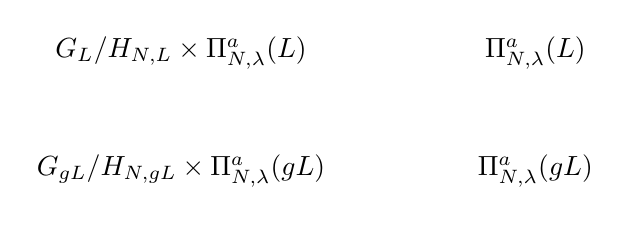
\begin{tikzpicture}[scale=1.5, baseline = -0.5ex]
\node (A) at (0,1) {$G_L/{H_{N,L}}\times\Pi_{N,\lambda}^a(L)$};
\node (B) at (3,1) {$\Pi_{N,\lambda}^a(L)$};
\node (C) at (0,0) {$G_{gL}/{H_{N,gL}}\times\Pi_{N,\lambda}^a(gL)$};
\node (D) at (3,0) {$\Pi_{N,\lambda}^a(gL)$};

\cdarrow (A) edge (B);
\cdarrow (A) edge (C);
\cdarrow (B) edge (D);
\cdarrow (C) edge (D);
\end{tikzpicture}
\end{equation*}

\subsection{Incidence in affine flag varieties}

\begin{lemma}\label{lemma:incidence-varieties-main}
Given $N,a,b,c\in\naturals$, $\lambda,\mu\in\compositions$, $L\in\flags$ and $i,j\in\integers$,
\begin{equation*}
\left\{(L',L'')\in\Pi_{N,\lambda}^a(L)\times\Pi_{N,\mu}^b(L): \dim\left(\frac{L_i'}{L_i'\cap L_j''}\right)\le c\right\}
\end{equation*}
is a closed set in the projective variety $\Pi_{N,\lambda}^a(L)\times\Pi_{N,\mu}^b(L)$.
\end{lemma}

\begin{proof}
There is $M\geq N$ so that $\epsilon^M L_0\subset L_i'\subset\epsilon^{-M}L_0$ and $\epsilon^M L_0\subset L_j''\subset\epsilon^{-M}L_0$. Let $a'=a+(M-N)r$ and $b'=b+(M-N)r$. Lemma \ref{lemma:nesting-subvarieties} shows that $\Pi_{N,\lambda}^a(L)$ is a subvariety of $\Pi_{M,\lambda}^{a'}(L)$, so $\Pi_{N,\lambda}^a(L)\times\Pi_{N,\mu}^b(L)$ is a subvariety of $\Pi_{M,\lambda}^{a'}(L)\times\Pi_{M,\mu}^{b'}(L)$.

The fact that
\begin{equation*}
\dim\left(\frac{L_i'}{L_i'\cap L_j''}\right) = \dim\left(\frac{L_i'/{\epsilon^M L_0}}{L_i'/{\epsilon^M L_0}\cap L_j''/{\epsilon^M L_0}}\right),
\end{equation*}
together with Lemma \ref{lemma:projective-varieties-of-cyclic-flags} and Lemma \ref{lemma:grassmannian-incidence-varieties}, shows that
\begin{equation*}
\left\{(L',L'')\in\Pi_{M,\lambda}^{a'}(L)\times\Pi_{M,\mu}^{b'}(L):\dim\left(\frac{L_i'}{L_i'\cap L_j''}\right)\le c\right\}
\end{equation*}
is closed, so the intersection with $\Pi_{N,\lambda}^a(L)\times\Pi_{N,\mu}^b(L)$ is closed.
\end{proof}

\begin{lemma}\label{lemma:incidence-varieties-consequences}
Given $N,a,c\in\naturals$, $\lambda\in\compositions$, $L\in\flags$ and $i,j\in\integers$,
\begin{equation*}
\left\{L'\in\Pi_{N,\lambda}^a(L):\dim\left(\frac{L_i}{L_i\cap L_j'}\right)\le c\right\}
\end{equation*}
and
\begin{equation*}
\left\{L'\in\Pi_{N,\lambda}^a(L): \dim\left(\frac{L_j'}{L_i\cap L_j'}\right)\le c\right\}
\end{equation*}
are closed sets in $\Pi_{N,\lambda}^a(L)$.
\end{lemma}

\begin{proof}
This is a result of Lemma \ref{lemma:grassmannian-incidence-lemmas}, since
\begin{equation*}
\dim\left(\frac{L_i}{L_i\cap L_j'}\right) = \dim\left(\frac{L_i/{\epsilon^M L_0}}{L_i/{\epsilon^M L_0}\cap L_j'/{\epsilon^M L_0}}\right),
\end{equation*}
where $M\geq N$ is chosen so that $\epsilon^M L_0\subset L_i\subset\epsilon^{-M}L_0$ and $\epsilon^M L_0\subset L_j'\subset\epsilon^{-M}L_0$ for each $L'\in\Pi_{N,\lambda}^a(L)$.
\end{proof}


\section{Geometry of orbits}

Let $A\in\matrices$ and $L\in\flags_{\ro{A}}$ and write $\lambda=\co{A}$. Recall that
\begin{equation*}
\xprod[L]{A} = \{L'\in\flags_\lambda: (L,L')\in\orbit{A}\}.
\end{equation*}

\begin{lemma}\label{lemma:bounded-orbits}
There is $N\in\naturals$ such that $\xprod[L]{A}\subset\Pi_{N,\lambda}^a(L)$, where $a=d_{nN,0}{A}$.
\end{lemma}

\begin{proof}
There is $N\in\naturals$ so that $a_{i,j}=0$ whenever $|j-i|>nN$. If $(L,L')\in\orbit{A}$ then
\begin{equation*}
\dim\left(\frac{L_0'}{L_0'\cap\epsilon^{-N}L_0}\right) = \dim\left(\frac{L_0'}{L_0'\cap L_{nN}}\right) = \sum_{s>nN,t\le 0} a_{s,t} = 0,
\end{equation*}
so it follows $L_0'\subset\epsilon^{-N}L_0$. Similarly,
\begin{equation*}
\dim\left(\frac{\epsilon^N L_0}{\epsilon^N L_0\cap L_0'}\right) = \dim\left(\frac{L_{-nN}}{L_{-nN}\cap L_0'}\right) = \sum_{s\le -nN,t>0} a_{s,t} = 0,
\end{equation*}
which shows $\epsilon^N L_0\subset L_0'$. Moreover,
\begin{equation*}
\dim\left(\frac{\epsilon^{-N}L_0}{L_0'}\right) = \dim\left(\frac{\epsilon^{-N}L_0}{\epsilon^{-N}L_0\cap L_0'}\right) = \sum_{s\le nN,t>0}a_{s,t} = d_{nN,0}(A),
\end{equation*}
as a result of Lemma \ref{lemma:codimension-formula-corner-sums}. 
\end{proof}

Assume $N\in\naturals$ is chosen so that $\xprod[L]{A}\subset\Pi_{N,\lambda}^a(L)$, where $a=d_{nN,0}{A}$, as in Lemma \ref{lemma:bounded-orbits}.

\begin{lemma}\label{lemma:orbits-are-quasiprojective}
$\xprod[L]{A}$ is a locally closed subset of $\Pi_{N,\lambda}^a(L)$. In particular, $\xprod[L]{A}$ is a quasiprojective variety.
\end{lemma}

\begin{proof}
If $L'\in\Pi_{N,\lambda}^a(L)$ then
\begin{equation*}
L_{-Nn}=\epsilon^N L_0\subset L_0'\subset L_1'\subset L_n'\subset \epsilon^{-1-N}L_0 = L_{(N+1)n}.
\end{equation*}
Therefore $\xprod[L]{A}$ is the subset of $\Pi_{N,\lambda}^a(L)$ defined by the conditions $\dim(L_i/{L_i\cap L_j'})=d_{i,j}{A}$ for $i:-Nn\le i<j$ and $\dim(L_j'/{L_i\cap L_j'})=\bar{d}_{i,j}{A}$ for $i:j<i\le(N+1)n$, for $j=1,\ldots,n$.

The set of $L'\in\Pi_{N,\lambda}^a(L)$ with $\dim(L_i/{L_i\cap L_j'})\le d_{i,j}{A}$ for $j=1,\ldots,n$ and $i:-Nn\le i<j$ and $\dim(L_j'/{L_i\cap L_j'})\le\bar{d}_{i,j}{A}$ for $j=1,\ldots,n$ and $i:j<i\le(N+1)n$ is a closed subset of $\Pi_{N,\lambda}^a(L)$, as a result of Lemma \ref{lemma:incidence-varieties-consequences}.

On the other hand, the set of $L'\in\Pi_{N,\lambda}^a(L)$ satisfying the conditions $\dim(L_i/{L_i\cap L_j'})\geq d_{i,j}{A}$ (for $i<j$) and $\dim(L_j'/{L_i\cap L_j'})\geq\bar{d}_{i,j}{A}$ (for $i>j$) is open in $\Pi_{N,\lambda}^a(L)$ since the complement is closed, as a result of Lemma \ref{lemma:incidence-varieties-consequences}.

Therefore $\xprod[L]{A}$ is the intersection of an open set and a closed set in $\Pi_{N,\lambda}^a(L)$, so $\xprod[L]{A}$ is locally closed. It follows that $\xprod[L]{A}$ is an open subset of the projective variety $\overline{\xprod[L]{A}}$, so is a quasiprojective variety as claimed.
\end{proof}

\begin{lemma}\label{lemma:orbits-are-irreducible}
$\xprod[L]{A}$ is irreducible.
\end{lemma}

\begin{proof}
For any $L'\in\xprod[L]{A}$, $\xprod[L]{A} = G_L/{H_{N,L}}\cdot L'$. Lemma \ref{lemma:connected-algebraic-group} shows that $G_L/{H_{N,L}}$ is a connected algebraic group which acts algebraically on $\Pi_{N,\lambda}^a(L)$. The image of $G_L/{H_{N,L}}$ under the morphism $g\mapsto gL'$ equals $\xprod[L]{A}$, which shows $\xprod[L]{A}$ is irreducible since $G_L/{H_{N,L}}$ is irreducible.
\end{proof}

Consequently, $\overline{\xprod[L]{A}}$ is an irreducible projective variety and the action of $G_L/{H_{N,L}}$ on $\Pi_{N,\lambda}^a(L)$ restricts to an algebraic group action on $\overline{\xprod[L]{A}}$ for which there are finitely many orbits. In particular, $\overline{\xprod[L]{A}}\setminus\xprod[L]{A}$ is a union of finitely many orbits which are so-called degenerations of the orbit $\xprod[L]{A}$.


\section{Geometry of orbit products}

Let $A,B\in\matrices$ with $\co{A}=\ro{B}$ and write $\lambda=\co{A}$ and $\mu=\co{B}$. Fix $L\in\flags_{\ro{A}}$. Recall

\begin{equation*}
\yprod[L]{A,B}=\{(L',L'')\in\flags_{\lambda}\times\flags_{\mu}: L'\in\xprod[L]{A}, L''\in\xprod[L']{B}\}
\end{equation*}
and
\begin{equation*}
\xprod[L]{A,B}=\{L''\in\flags_{\mu}: \exists L'\in\xprod[L]{A} \text{ with } L''\in\xprod[L']{B}\}
\end{equation*}

\begin{lemma}\label{lemma:embedding-orbit-products}
There is $N\in\naturals$ such that
\begin{equation*}
\yprod[L]{A,B}\subset\Pi_{N,\lambda}^a(L)\times\Pi_{2N,\mu}^{a+b}(L),
\end{equation*}
where $a=d_{nN,0}{(A)}$ and $b=d_{nN,0}{(B)}$.
\end{lemma}

\begin{proof}
There is $N\in\naturals$ such that $\epsilon^N{L_0}\subset L_0'\subset\epsilon^{-N}L_0$ and $\epsilon^NL_0'\subset L_0''\subset\epsilon^{-N}L_0'$ for each $(L',L'')\in\yprod[L]{A,B}$, using Lemma \ref{lemma:bounded-orbits}. Set $a=d_{nN,0}{(A)}$ and $b=d_{nN,0}{(B)}$.

Then for any $(L',L'')\in\yprod[L]{A,B}$,
\begin{equation*}
\epsilon^{2N}L_0\subset\epsilon^NL_0'\subset L_0''\subset\epsilon^{-N}L_0'\subset\epsilon^{-2N}L_0
\end{equation*}
and
\begin{align*}
\dim\left(\frac{\epsilon^{-2N}L_0}{L_0''}\right)
&=\dim\left(\frac{\epsilon^{-N}L_0'}{L_0''}\right) + \dim\left(\frac{\epsilon^{-2N}L_0}{\epsilon^{-N}L_0'}\right)\\
&=\dim\left(\frac{\epsilon^{-N}L_0'}{L_0''}\right) + \dim\left(\frac{\epsilon^{-N}L_0}{L_0'}\right)\\
&= a+b,
\end{align*}
as a result of Lemma \ref{lemma:codimension-formula-corner-sums}, so $(L',L'')\in\Pi_{N,\lambda}^a(L)\times\Pi_{2N,\mu}^{a+b}(L)$ as required.
\end{proof}

Now assume $N\in\naturals$ is chosen so that $\yprod[L]{A,B}\subset\Pi_{N,\lambda}^a(L)\times\Pi_{2N,\mu}^{a+b}(L)$, where $a=d_{nN,0}{(A)}$ and $b=d_{nN,0}{(B)}$, using Lemma \ref{lemma:embedding-orbit-products}.

\begin{lemma}\label{lemma:y-prod-is-quasiprojective}
$\yprod[L]{A,B}$ is a locally closed subset of $\Pi_{N,\lambda}^a(L)\times\Pi_{2N,\mu}^{a+b}(L)$. In particular, $\yprod[L]{A,B}$ is a quasiprojective variety.
\end{lemma}

\begin{proof}
$\yprod[L]{A,B}$ is the subset of $\Pi_{N,\lambda}^a(L)\times\Pi_{2N,\mu}^{a+b}(L)$ consisting of those $(L',L'')$ satisfying the following conditions: $\dim(L_i/{L_i\cap L_j'}) = d_{i,j}{(A)}$ for $i<j$, $\dim(L_j'/{L_i\cap L_j'})=\bar{d}_{i,j}{(A)}$ for $i>j$, $\dim(L_i'/{L_i'\cap L_j''})=d_{i,j}{(B)}$ for $i<j$ and $\dim(L_j''/{L_i'\cap L_j''})=\bar{d}_{i,j}{(B)}$. Only finitely many conditions are required to define $\yprod[L]{A,B}$ since there are only finitely many nonzero entries in $A$ and $B$ modulo the $(n,n)$-periodicity.

The conditions $\dim(L_i/{L_i\cap L_j'})\le d_{i,j}{(A)}$, $\dim(L_i'/{L_i'\cap L_j''})\le d_{i,j}{(B)}$, $\dim(L_j'/{L_i\cap L_j'})\le\bar{d}_{i,j}{(A)}$ and $\dim(L_j''/{L_i'\cap L_j''})\le\bar{d}_{i,j}{(B)}$ define closed subsets of $\Pi_{N,\lambda}^a(L)\times\Pi_{2N,\mu}^{a+b}(L)$ for each $i,j\in\integers$, as a result of Lemma \ref{lemma:incidence-varieties-main} and Lemma \ref{lemma:incidence-varieties-consequences}.

On the other hand, the conditions $\dim(L_i/{L_i\cap L_j'})\geq d_{i,j}{(A)}$, $\dim(L_i'/{L_i'\cap L_j''})\geq d_{i,j}{(B)}$, $\dim(L_j'/{L_i\cap L_j'})\geq\bar{d}_{i,j}{(A)}$ and $\dim(L_j''/{L_i'\cap L_j''})\geq\bar{d}_{i,j}{(B)}$ define open subsets of $\Pi_{N,\lambda}^a(L)\times\Pi_{2N,\mu}^{a+b}(L)$ for each $i,j\in\integers$, using Lemma \ref{lemma:incidence-varieties-main} and Lemma \ref{lemma:incidence-varieties-consequences}.

Therefore $\yprod[L]{A,B}$ is the intersection of finitely many open sets and finitely many closed sets in $\Pi_{N,\lambda}^a(L)\times\Pi_{2N,\mu}^{a+b}(L)$, so $\yprod[L]{A,B}$ is locally closed. In particular, $\yprod[L]{A,B}$ is a quasiprojective variety.
\end{proof}

\begin{lemma}\label{lemma:yprod-as-a-saturation}
For any $L'\in\xprod[L]{A}$, $\yprod[L]{A,B} = G_L\cdot(\{L'\}\times\xprod[L']{B})$.
\end{lemma}

\begin{proof}
Let $L'\in\xprod[L]{A}$, then $\{L'\}\times\xprod[L']{B}$ is contained in $\yprod[L]{A,B}$ and $G_L$ acts on $\yprod[L]{A,B}$, so $G_L\cdot(\{L'\}\times\xprod[L']{B})$ is contained in $\yprod[L]{A,B}$. If $(N',N'')\in\yprod[L]{A,B}$, then $N'=\sigma L'$ for some $\sigma\in G_L$, since $N'\in\xprod[L]{A}$. Then $(N',N'')=\sigma (L',\sigma^{-1}N'')$ and $\sigma^{-1}N''\in\xprod[\sigma^{-1}N']{B}=\xprod[L']{B}$, so $(N',N'')\in\sigma\cdot(\{L'\}\times\xprod[L']{B})$. Therefore $\yprod[L]{A,B}=G_L\cdot(\{L'\}\times\xprod[L']{B})$ as claimed.
\end{proof}

\begin{proposition}\label{prop:irreducible-y-prod}
$\yprod[L]{A,B}$ is irreducible.
\end{proposition}

\begin{proof}
Let $L'\in\xprod[L]{A}$. $G_L/{H_{2N,L}}$ is a connected algebraic group acting algebraically on $\Pi_{N,\lambda}^a(L)\times\Pi_{2N,\mu}^{a+b}(L)$ by Lemma \ref{lemma:connected-algebraic-group}. $\xprod[L']{B}$ is an irreducible locally closed subset of $\Pi_{2N,\mu}^{a+b}(L)$, so $\{L'\}\times\xprod[L']{B}$ is an irreducible locally closed set in $\Pi_{N,\lambda}^a(L)\times\Pi_{2N,\mu}^{a+b}(L)$. $\yprod[L]{A,B}=G_L\cdot (\{L'\}\times\xprod[L']{B}) = G_L/{H_{2N,L}}\cdot (\{L'\}\times\xprod[L']{B})$, by Lemma \ref{lemma:yprod-as-a-saturation}, so it follows that $\yprod[L]{A,B}$ is irreducible.
\end{proof}

Let $p_2$ be the projection onto the second factor $\Pi_{N,\lambda}^a(L)\times\Pi_{2N,\mu}^{a+b}(L)\to\Pi_{2N,\mu}^{a+b}(L)$. $p_2$ is a closed morphism since $\Pi_{N,\lambda}^a(L)$ is a projective variety and therefore complete, by Lemma \ref{lemma:projective-varieties-of-cyclic-flags}. Therefore $p_2(\overline{\yprod[L]{A,B}})=\overline{\xprod[L]{A,B}}$, since $p_2(\yprod[L]{A,B})=\xprod[L]{A,B}$.

\begin{lemma}\label{lemma:irreducible-x-prod}
$\xprod[L]{A,B}$ is irreducible and constructible.
\end{lemma}

\begin{proof}
Proposition \ref{prop:irreducible-y-prod} shows that $\yprod[L]{A,B}$ is irreducible and locally closed, so it follows $\xprod[L]{A,B}$ is irreducible and constructible, since $\xprod[L]{A,B}=p_2(\yprod[L]{A,B})$.
\end{proof}

\begin{proposition}\label{prop:open-orbit-x-prod}
There is a unique open $G_L$-orbit in $\xprod[L]{A,B}$.
\end{proposition}

\begin{proof}
$\xprod[L]{A,B}$ consists of finitely many $G_L$-orbits and is an irreducible topological space, by Lemma \ref{lemma:irreducible-x-prod}. Consequently, $\xprod[L]{C}$ is dense in $\xprod[L]{A,B}$ for some $C\in\matrices^{A,B}$. Lemma \ref{lemma:orbits-are-quasiprojective} shows that $\xprod[L]{C}$ is locally closed in $\xprod[L]{A,B}$, so $\xprod[L]{C}$ is open in $\overline{\xprod[L]{C}}=\xprod[L]{A,B}$. Irreducibility of $\xprod[L]{A,B}$ shows that there is a unique open $G_L$-orbit, since two nonempty open sets in $\xprod[L]{A,B}$ intersect nontrivially, thus any two open $G_L$ orbits in $\xprod[L]{A,B}$ coincide.
\end{proof}

Let $A\ast B\in\matrices$ be the matrix corresponding to the dense open $G_L$-orbit in $\xprod[L]{A,B}$, so $\overline{\xprod[L]{A\ast B}}=\overline{\xprod[L]{A,B}}$.

\section{Degenerations of orbits and the combinatorial partial order}

\begin{theorem}\label{theorem:compare-partial-orders}
Let $A,B\in\matrices$ with $\ro{A}=\ro{B}$ and $\co{A}=\co{B}$, then $B\le A$ if and only if $\xprod[L]{B}\subset\overline{\xprod[L]{A}}$ for any $L\in\flags_{\ro{A}}$.
\end{theorem}

\begin{proof}
Let $\lambda=\co{A}$, $\mu=\ro{A}$ and fix $L\in\flags_\mu$. Assume $N\in\naturals$ is chosen so that $\xprod[L]{A}\subset\Pi_{N,\lambda}^a(L)$ and $\xprod[L]{B}\subset\Pi_{N,\lambda}^b(L)$, where $a=d_{nN,0}{(A)}$ and $b=d_{nN,0}{(B)}$. Then $\xprod[L]{A}$ is an open subset of the projective variety consisting of those $L'\in\Pi_{N,\lambda}^a(L)$ such that
\begin{equation*}
\dim\left(\frac{L_i}{L_i\cap L_j'}\right)\le d_{i,j}{(A)}
\end{equation*}
and
\begin{equation*}
\dim\left(\frac{L_j'}{L_i\cap L_j'}\right)\le\bar{d}_{i,j}{(A)},
\end{equation*}
for all $i,j\in\integers$.

Assume $\xprod[L]{B}\subset \overline{\xprod[L]{A}}$, then
\begin{equation*}
d_{i,j}{(B)} = \dim\left(\frac{L_i}{L_i\cap L_j'}\right) \le d_{i,j}{(A)}
\end{equation*}
and
\begin{equation*}
\bar{d}_{i,j}{(B)} = \dim\left(\frac{L_j'}{L_i\cap L_j'}\right) \le \bar{d}_{i,j}{(A)},
\end{equation*}
for each $i,j\in\integers$, for any $L'\in\xprod[L]{B}$. So $B\le A$ if $\xprod[L]{B}\le\overline{\xprod[L]{A}}$.

{\color{red}
Conversely, suppose $A\le B$.
}

\end{proof}

\begin{corollary}
The maximum in $\matrices^{A,B}$ is $A\ast B$.
\end{corollary}



\section{Associativity of the generic product}

Let $A,B,C\in\matrices$ with $\co{A}=\ro{B}$ and $\co{B}=\ro{C}$ and fix $L\in\flags_{\ro{A}}$. Write $\lambda=\co{A}$, $\mu=\co{B}$ and $\nu=\co{C}$. Define
\begin{equation*}
\yprod[L]{A,B,C} = \left\{(L',L'',L''')\in\flags^3: L'\in\xprod[L]{A}, L''\in\xprod[L']{B}, L'''\in\xprod[L'']{C}\right\}
\end{equation*}
and
\begin{equation*}
\xprod[L]{A,B,C} = \left\{L'''\in\flags: \exists (L',L'')\in\flags^2 \text{ with } (L',L'',L''')\in\yprod[L]{A,B,C}\right\}.
\end{equation*}

\begin{lemma}\label{lemma:embedding-y-triple}
There is $N\in\naturals$ such that $\yprod[L]{A,B,C}$ is contained in $\Pi_{N,\lambda}^a(L)\times\Pi_{2N,\mu}^{a+b}(L)\times\Pi_{3N,\nu}^{a+b+c}(L)$, where $a=d_{nN,0}{(A)}$, $b=d_{nN,0}{(B)}$ and $c=d_{nN,0}{(C)}$.
\end{lemma}

\begin{proof}
Lemma \ref{lemma:bounded-orbits} shows that there is $N\in\naturals$ such that $\epsilon^N L_0\subset L_0'\subset\epsilon^{-N}L_0$, $\epsilon^N L_0'\subset L_0''\subset\epsilon^{-N}L_0'$ and $\epsilon^N L_0''\subset L_0'''\subset\epsilon^{-N}L_0''$ for each $(L',L'',L''')\in\yprod[L]{A,B,C}$. Using the proof of Lemma \ref{lemma:embedding-orbit-products}, it follows $L''\in\Pi_{2N,\mu}^{a+b}(L)$ and $L'''\in\Pi_{2N,\nu}^{b+c}(L')\subset\Pi_{3N,\nu}^{a+b+c}(L)$.
\end{proof}

Assume $N\in\naturals$ is chosen so that $\yprod[L]{A,B,C}\subset\Pi_{N,\lambda}^a(L)\times\Pi_{2N,\mu}^{a+b}(L)\times\Pi_{3N,\nu}^{a+b+c}(L)$, where $a=d_{nN,0}{(A)}$, $b=d_{nN,0}{(B)}$ and $c=d_{nN,0}{(C)}$, as in Lemma \ref{lemma:embedding-y-triple}.

\begin{lemma}\label{lemma:y-triple-is-quasiprojective}
$\yprod[L]{A,B,C}$ is a locally closed subset of $\Pi_{N,\lambda}^a(L)\times\Pi_{2N,\mu}^{a+b}(L)\times\Pi_{3N,\nu}^{a+b+c}(L)$. In particular, $\yprod[L]{A,B,C}$ is a quasiprojective variety.
\end{lemma}

\begin{proof}
Write $\Pi=\Pi_{N,\lambda}^a(L)\times\Pi_{2N,\mu}^{a+b}(L)\times\Pi_{3N,\nu}(L)$. Then $\yprod[L]{A,B,C}$ consists of those $(L',L'',L''')\in\Pi$ satisfying the following conditions:
\begin{align}
\dim\left(\frac{L_i}{L_i\cap L_j'}\right) &= d_{i,j}{(A)},\\
\dim\left(\frac{L_i'}{L_i'\cap L_j''}\right) &= d_{i,j}{(B)},\\
\dim\left(\frac{L_i''}{L_i''\cap L_j'''}\right) &= d_{i,j}{(C)},
\end{align}
for $(i,j)\in \{1,\ldots,n\}\times\integers$ with $i<j<(N+1)n$, and
\begin{align}
\dim\left(\frac{L_j'}{L_i\cap L_j'}\right) &= \bar{d}_{i,j}{(A)},\\
\dim\left(\frac{L_j''}{L_i'\cap L_j''}\right) &= \bar{d}_{i,j}{(B)},\\
\dim\left(\frac{L_j'''}{L_i''\cap L_j'''}\right) &= \bar{d}_{i,j}{(C)},
\end{align}
for $(i,j)\in \{1,\ldots,n\}\times\integers$ with $-Nn<j<i$.

For $i<j$, the conditions
\begin{align*}
\dim\left(L_i/{L_i\cap L_j'}\right)&\le d_{i,j}{(A)},\\
\dim\left(L_i'/{L_i'\cap L_j''}\right)&\le d_{i,j}{(B)}
\end{align*}
and
\begin{equation*} 
\dim\left(L_i''/{L_i''\cap L_j'''}\right)\le d_{i,j}{(C)}
\end{equation*}
define closed subsets of $\Pi$, by Lemma \ref{lemma:incidence-varieties-main}. For $i>j$, the conditions
\begin{align*}
\dim\left(L_j'/{L_i\cap L_j'}\right)&\le \bar{d}_{i,j}{(A)},\\
\dim\left(L_j''/{L_i'\cap L_j''}\right)&\le \bar{d}_{i,j}{(B)}
\end{align*}
and
\begin{equation*}
\dim\left(L_j'''/{L_i''\cap L_j'''}\right)\le \bar{d}_{i,j}{(C)}
\end{equation*}
also define closed subsets of $\Pi$.

On the other hand, the conditions $\dim\left(L_i/{L_i\cap L_j'}\right)\geq d_{i,j}{(A)}$, $\dim\left(L_i'/{L_i'\cap L_j''}\right)\geq d_{i,j}{(B)}$ and $\dim\left(L_i''/{L_i''\cap L_j'''}\right)\geq d_{i,j}{(C)}$ for $i<j$ define open subsets of $\Pi$. Similarly, the conditions $\dim\left(L_j'/{L_i\cap L_j'}\right)\geq \bar{d}_{i,j}{(A)}$, $\dim\left(L_j''/{L_i'\cap L_j''}\right)\geq \bar{d}_{i,j}{(B)}$ and $\dim\left(L_j'''/{L_i''\cap L_j'''}\right)\geq \bar{d}_{i,j}{(C)}$ for $i>j$ define open subsets of $\Pi$.

Therefore $\yprod[L]{A,B,C}$ is the intersection of finitely many closed sets in $\Pi$ with finitely many open subsets of $\Pi$, so $\yprod[L]{A,B,C}$ is locally closed. In particular, $\yprod[L]{A,B,C}$ is a quasiprojective variety.
\end{proof}

\begin{lemma}\label{lemma:y-triple-stabilisers}
For any $(L',L'',L''')\in\yprod[L]{A,B,C}$,
\begin{equation*}
\yprod[L]{A,B,C} = \left\{ \alpha\cdot (L',\beta L'',\beta\gamma L'''): \alpha\in G_L, \beta\in G_{L'}, \gamma\in G_{L''}\right\}.
\end{equation*}
In particular,
\begin{equation*}
\yprod[L]{A,B,C} = G_L\cdot\left(\{L'\}\times\yprod[L']{B,C}\right)
\end{equation*}
for each $L'\in\xprod[L]{A}$.
\end{lemma}

\begin{proof}
Let $(L',L'',L''')\in\yprod[L]{A,B,C}$. Given $\alpha\in G_{L}$, $\beta\in G_{L'}$ and $\gamma\in G_{L''}$, $(\alpha L',\alpha\beta L'', \alpha\beta\gamma L''')$ is in $\yprod[L]{A,B,C}$ since
\begin{align*}
(L,\alpha L') &= \alpha (L,L')\in\orbit{A}\\
(\alpha L', \alpha\beta L'') &= \alpha\beta (L',L'')\in\orbit{B}\\
(\alpha\beta L'',\alpha\beta\gamma L''') &= \alpha\beta\gamma (L'',L''')\in\orbit{C}
\end{align*}

For each $(N',N'',N''')\yprod[L]{A,B,C}$ there exist $\sigma_1,\sigma_2,\sigma_3\in G$ with
\begin{align*}
(L,N') &= \sigma_1(L,L')\\
(N',N'') &= \sigma_2(L',L'')\\
(N'',N''') &= \sigma_3(L'',L''').
\end{align*}

Let $\alpha = \sigma_1$, $\beta = \sigma_1^{-1}\sigma_2$ and $\gamma = \sigma_2^{-1}\sigma_3$, so $\sigma_2=\alpha\beta$ and $\sigma_3=\alpha\beta\gamma$. It follows that
\begin{equation*}
(N',N'',N''') = (\alpha L',\alpha\beta L'', \alpha\beta\gamma L'''),
\end{equation*}
which proves the first claim. The second claim follows from the first since $(L'',L''')\in\yprod[L']{B,C}$ and therefore
\begin{equation*}
\yprod[L']{B,C} = \{(\beta L'',\beta\gamma L'''):\beta\in G_{L'}, \gamma\in G_{L''}\},
\end{equation*}
as required.
\end{proof}

\begin{proposition}\label{proposition:irreducible-y-triple}
$\yprod[L]{A,B,C}$ is irreducible.
\end{proposition}

\begin{proof}
Write
\begin{equation*}
\Pi=\Pi_{N,\lambda}^{a}(L)\times\Pi_{2N,\mu}^{a+b}(L)\times\Pi_{3N,\nu}^{a+b+c}(L).
\end{equation*}

Lemma $\ref{lemma:projective-varieties-of-cyclic-flags}$ shows that $\Pi$ is a projective algebraic variety and Lemma \ref{lemma:connected-algebraic-group} shows that $G_L/{H_{3N,L}}$ is a connected algebraic group acting algebraically on $\Pi$ by the diagonal action.

Let $L'\in\xprod[L]{A}$. As a result of Lemma \ref{lemma:y-triple-stabilisers} 
\begin{align*}
\yprod[L]{A,B,C}
&= G_L\cdot (\{L'\}\times\yprod[L']{B,C})\\
&= G_L/{H_{3N,L}}\cdot (\{L'\}\times\yprod[L']{B,C}).
\end{align*}

Proposition \ref{prop:irreducible-y-prod} shows that $\yprod[L']{B,C}$ is irreducible, so $\{L'\}\times\yprod[L']{B,C}$ is irreducible. The image of $\{L'\}\times\yprod[L']{B,C}$ under the action of $G_L/{H_{3N,L}}$ is irreducible, since $G_L/{H_{3N,L}}$ is connected and therefore irreducible. Therefore $\yprod[L]{A,B,C}$ is irreducible.
\end{proof}

Let $p_3$ be the projection of $\Pi_{N,\lambda}^a(L)\times\Pi_{2N,\mu}^{a+b}(L)\times\Pi_{3N,\nu}^{a+b+c}(L)$ onto the third factor. By the completeness property of projective varieties, $p_3$ is a closed morphism. The image of $\yprod[L]{A,B,C}$ under $p_3$ is $\xprod[L]{A,B,C}$, so $p_3(\overline{\yprod[L]{A,B,C}}) = \overline{\xprod[L]{A,B,C}}$.

\begin{lemma}\label{lemma:irreducible-x-triple}
$\xprod[L]{A,B,C}$ is irreducible and constructible.
\end{lemma}

\begin{proof}
Lemma \ref{lemma:y-triple-is-quasiprojective} and Proposition \ref{proposition:irreducible-y-triple} show that $\yprod[L]{A,B,C}$ is locally closed and irreducible. It follows $\xprod[L]{A,B}$ is irreducible and constructible, since $\xprod[L]{A,B,C}$ is the image of $\yprod[L]{A,B,C}$ under the morphism $p_3$.
\end{proof}

\begin{lemma}\label{lemma:generic-triple-product}
There is a unique open and dense $G_L$-orbit in $\xprod[L]{A,B,C}$.
\end{lemma}

\begin{proof}
There are only finitely many $G_L$-orbits in $\xprod[L]{A,B,C}$. In particular,
\begin{equation*}
\xprod[L]{A,B,C}=\bigcup_{D\in\matrices^{A,B}}\xprod[L]{D,C}=\bigcup_{D\in\matrices^{A,B}}\bigcup_{D'\in\matrices^{D,C}}\xprod[L]{D'}
\end{equation*}
and
\begin{equation*}
\overline{\xprod[L]{A,B,C}} = \bigcup_{D\in\matrices^{A,B}}\bigcup_{D'\in\matrices^{D,C}}\overline{\xprod[L]{D'}}.
\end{equation*}
There is $D\in\matrices$ such that $\overline{\xprod[L]{D}}=\overline{\xprod[L]{A,B,C}}$, since $\xprod[L]{A,B,C}$ is irreducible, by Lemma \ref{lemma:irreducible-x-triple}. By Lemma \ref{lemma:orbits-are-quasiprojective}, $\xprod[L]{D}$ is open in $\overline{\xprod[L]{D}}=\overline{\xprod[L]{A,B,C}}$, so $\xprod[L]{D}$ is open in $\xprod[L]{A,B,C}$.

If $\xprod[L]{D}$ and $\xprod[L]{D'}$ are open in $\xprod[L]{A,B,C}$, then $\xprod[L]{D}$ and $\xprod[L]{D'}$ have nonempty intersection since $\xprod[L]{A,B,C}$ is irreducible, then $\xprod[L]{D}=\xprod[L]{D'}$.
\end{proof}

\begin{lemma}\label{lemma:yprod-generic-A-B}
$p_3^{-1}(\xprod[L]{A\ast B,C})$ is open in $\overline{\yprod[L]{A,B,C}}$.
\end{lemma}

\begin{proof}
Projection onto the second component is a closed morphism of varieties $p_2\colon\overline{\yprod[L]{A,B,C}}\to\overline{\xprod[L]{A,B}}$ with $p_2(\yprod[L]{A,B,C})=\xprod[L]{A,B}$. It follows that $p_3^{-1}(\xprod[L]{A\ast B,C})$ is open in $\overline{\yprod[L]{A,B,C}}$ since $p_3^{-1}(\xprod[L]{A\ast B,C})=p_2^{-1}(\xprod[L]{A\ast B})$ and $\xprod[L]{A\ast B}$ is open in $\overline{\xprod[L]{A,B}}$.
\end{proof}

\begin{lemma}\label{lemma:yprod-generic-B-C}
$p_3^{-1}(\xprod[L]{A,B\ast C})$ is open in $\overline{\yprod[L]{A,B,C}}$.
\end{lemma}

\begin{proof}
$p_3^{-1}(\xprod[L]{A,B\ast C})$ consists of those $(L',L'',L''')\in\overline{\yprod[L]{A,B,C}}$ such that $\dim\left(L_i'/{L_i'\cap L_j'''}\right)\geq d_{i,j}(B\ast C)$ for $i<j$ and $\dim\left(L_j'''/{L_i'\cap L_j'''}\right)\geq\bar{d}_{i,j}(B\ast C)$ for $i>j$. Each of these conditions defines an open subset of $\overline{\yprod[L]{A,B,C}}$ as a result of Lemma \ref{lemma:incidence-varieties-main} and only finitely many conditions are required to determine $p_3^{-1}(\xprod[L]{A,B\ast C})$, as before. Therefore $p_3^{-1}(\xprod[L]{A,B\ast C})$ is the intersection of finitely many open sets in $\overline{\yprod[L]{A,B,C}}$, so is open as claimed.
\end{proof}

\begin{proposition}\label{proposition:associativity}
$\xprod[L]{A\ast (B\ast C)} = \xprod[L]{(A\ast B)\ast C}$.
\end{proposition}

\begin{proof}
The unique open $G_L$-orbit in $\xprod[L]{A\ast B, C}$ is $\xprod[L]{(A\ast B)\ast C}$, so $p_3^{-1}(\xprod[L]{(A\ast B)\ast C})$ is open in $p_3^{-1}(\xprod[L]{A\ast B,C})$. Lemma \ref{lemma:yprod-generic-A-B} shows that $p_3^{-1}(\xprod[L]{A\ast B,C})$ is open in $\overline{\yprod[L]{A,B,C}}$, so $p_3^{-1}(\xprod[L]{(A\ast B)\ast C})$ is open in $\overline{\yprod[L]{A,B,C}}$.

Similarly, $\xprod[L]{A\ast (B\ast C)}$ is open in $\xprod[L]{A,B\ast C}$, so $p_3^{-1}(\xprod[L]{A\ast (B\ast C)})$ is open in $p_3^{-1}(\xprod[L]{A,B\ast C})$. Lemma \ref{lemma:yprod-generic-B-C} shows that $p_3^{-1}(\xprod[L]{A,B\ast C})$ is open in $\overline{\yprod[L]{A,B,C}}$, so it follows $p_3^{-1}(\xprod[L]{A\ast (B\ast C)})$ is open in $\overline{\yprod[L]{A,B,C}}$.

Therefore $f^{-1}(\xprod[L]{A\ast (B\ast C)})$ has nonempty intersection with $f^{-1}(\xprod[L]{(A\ast B)\ast C})$, since $\yprod[L]{A,B,C}$ is irreducible by Proposition \ref{proposition:irreducible-y-triple}. It follows that the $G_L$-orbits $\xprod[L]{A\ast (B\ast C)}$ and $\xprod[L]{(A\ast B)\ast C}$ have nonempty intersection and therefore $\xprod[L]{A\ast (B\ast C)}$ equals $\xprod[L]{(A\ast B)\ast C}$.
\end{proof}


\section{The generic affine algebra}

The generic affine algebra of rank $r$ and period $n$, denoted by $\generic$, is a free $\integers$-module with basis $\{e_A:A\in\matrices\}$ and $\integers$-bilinear multiplication given by
\begin{equation*}
e_A\ast e_B = e_{A\ast B}
\end{equation*}
for $A,B\in\matrices$ with $\co{A}=\ro{B}$, and
\begin{equation*}
e_A\ast e_B = 0
\end{equation*}
for $A,B\in\matrices$ with $\co{A}\neq\ro{B}$.

\begin{proposition}
The generic algebra $\generic$ is an associative $\integers$-algebra with $1$, with
\begin{equation*}
1=\sum_{\lambda\in\compositions} 1_\lambda
\end{equation*}
where
\begin{equation*}
1_\lambda = e_{D_\lambda},
\end{equation*}
for each $\lambda\in\compositions$.
\end{proposition}

\begin{proof}
Let $A,B,C\in\matrices$. If $\co{A}\neq\ro{B}$ or $\co{B}\neq\ro{C}$, then
\begin{equation*}
(e_A\ast e_B)\ast e_C = 0 = e_A\ast (e_B\ast e_C),
\end{equation*}
so we may now suppose $\co{A}=\ro{B}$ and $\co{B}=\ro{C}$.

As a result of Proposition \ref{proposition:associativity},
\begin{align*}
(e_A\ast e_B)\ast e_C &= e_{(A\ast B)\ast C}\\
&= e_{A\ast (B\ast C)}\\
&= e_A\ast (e_B\ast e_C),
\end{align*}
so it follows $\generic$ is an associative $\integers$-algebra.

The expression for the multiplicative identity follows from Lemma \ref{lemma:product-with-diagonal-orbits}, since
\begin{equation*}
e_A\ast \left(\sum_{\lambda\in\compositions} 1_\lambda\right) = e_A\ast 1_{\co{A}} = e_A
\end{equation*}
and
\begin{equation*}
\left(\sum_{\lambda\in\compositions} 1_\lambda\right)\ast e_A = 1_{\ro{A}}\ast e_A = e_A,
\end{equation*} 
for each $A\in\matrices$.
\end{proof}

\subsection{A categorical perspective}

\begin{proposition}\label{prop:generic-category}
The following constitutes a small category: the set of objects is $\compositions$ and the set of morphisms is $\matrices$. Given compositions $\lambda,\mu\in\compositions$, the morphisms with source $\mu$ and target $\lambda$ are those matrices $A\in\matrices$ with $\co{A}=\mu$ and $\ro{A}=\lambda$. Given $\lambda,\mu,\nu\in\compositions$ and $A,B\in\matrices$ with $\co{B}=\nu$, $\ro{B}=\mu=\co{A}$ and $\ro{A}=\lambda$, their composition is $A\ast B$, with source $\co{A\ast B}=\co{B}=\nu$ and target $\ro{A\ast B}=\ro{A}=\lambda$.
\end{proposition}

\begin{proof}
Proposition \ref{proposition:associativity} shows that the generic product $\ast$ is associative. For each object $\lambda\in\compositions$, the identity morphism $\lambda\to\lambda$ is the diagonal matrix $D_\lambda$.
\end{proof}

Then the generic affine algebra $\generic$ may be realised as the $\integers$-algebra of this category. Observe that there are only finitely many objects in this category and distinct objects are non-isomorphic, so the isomorphism classes in this category are in one to one correspondence with $\compositions$. The $\integers$-algebra of this category is the free $\integers$-module on $\matrices$ with $\integers$-bilinear multiplication given by the generic product $\ast$.



\chapter{A realisation of affine zero Schur algebras}

The purpose of this chapter is to study the link between the generic affine algebra $\generic$ to the affine $0$-Schur algebra $\zeroschur$.

The main result is the construction of an isomorphism of $\integers$-algebras from $\generic$ to $\zeroschur$ such that $E_i\mapsto E_i$, $F_j\mapsto F_j$ and $1_\lambda\mapsto 1_\lambda$, in the case that $n,r\geq 1$ with $r<n$.

\section{Preliminary results on the generic affine algebra}

Recall that the generic affine algebra $\generic$ is an associative $\integers$-algebra with a multiplicative basis $\{e_A:A\in\matrices\}$ over $\integers$, where
\begin{equation*}
e_A\ast e_B = e_{A\ast B}
\end{equation*}
for $A,B\in\matrices$ with $\co{A}=\ro{B}$, and
\begin{equation*}
e_A\ast e_B = 0
\end{equation*}
for $A,B\in\matrices$ with $\co{A}\neq\ro{B}$.

\subsection{Elementary basis elements}

For $i\in\{1,\ldots,n\}$ and $\lambda\in\compositions$ such that $\lambda_{i+1}>0$, define
\begin{equation*}
E_{i,\lambda} = e_{D_\lambda + \elem{i}{i+1} - \elem{i+1}{i+1}}
\end{equation*}
and let
\begin{equation*}
E_i = \sum_{\lambda\in\compositions:\lambda_{i+1}>0} E_{i,\lambda}
\end{equation*}
for each $i\in\{1,\ldots,n\}$

For $i\in\{1,\ldots,n\}$ and $\lambda\in\compositions$ such that $\lambda_i>0$, define
\begin{equation*}
F_{i,\lambda} = e_{D_\lambda + \elem{i+1}{i} - \elem{i}{i}}
\end{equation*}
and let
\begin{equation*}
F_i = \sum_{\lambda\in\compositions:\lambda_i>0} F_{i,\lambda}
\end{equation*}
for each $i\in\{1,\ldots,n\}$.

\begin{lemma}\label{lemma:fundamental-multiplication-rule-generic}
Let $i\in\{1,\ldots,n\}$ and $A\in\matrices$ and write $\mu=\ro{A}$.

If $\mu_{i+1}=0$ then $E_i\ast e_A=0$. If $\mu_{i+1}>0$, then
\begin{equation*}
E_i\ast e_A = e_{A+\elem{i}{p}-\elem{i+1}{p}},
\end{equation*}
where
\begin{equation*}
p=\max\{j\in\integers:a_{i+1,j}>0\}.
\end{equation*}

If $\mu_i=0$ then $F_i\ast e_A=0$. If $\mu_i>0$ then
\begin{equation*}
F_i\ast e_A = e_{A+\elem{i+1}{q}-\elem{i}{q}},
\end{equation*}
where
\begin{equation*}
q=\min\{j\in\integers: a_{i,j}>0\}.
\end{equation*}
\end{lemma}

\begin{proof}
Suppose $\mu_{i+1}>0$. Recall that the corresponding product in the affine $q$-Schur algebra $\qschur$ is
\begin{equation*}
E_i\cdot e_A = \sum_{j\in\integers:a_{i+1,j}>0} q^{\sum_{t>j} a_{i,t}}\qint{a_{i,j}+1}e_{A+\elem{i}{j}-\elem{i+1}{j}},
\end{equation*}
by Lemma \ref{lemma:fundamental-multiplication-rule}.

Suppose $B\in\matrices$ with $B=A+\elem{i}{j}-\elem{i+1}{j}$ for some $j\in\integers$. For $s\in\{1,\ldots,n\}$ and $t\in\integers$,
\begin{equation*}
d_{s,t}{(B)} = \begin{cases}
d_{s,t}{(A)} + 1 &: s=i \text{ and } t<j,\\
d_{s,t}{(A)} &: \text{ otherwise,}
\end{cases}
\end{equation*}
and
\begin{equation*}
\bar{d}_{s,t}{(B)} = \begin{cases}
\bar{d}_{s,t}{(A)} - 1 &: s=i \text{ and } t\geq j,\\
\bar{d}_{s,t}{(A)} &: \text{ otherwise.}
\end{cases}
\end{equation*}

It follows that if $j'<j$, then
\begin{equation*}
A+\elem{i}{j'}-\elem{i+1}{j'} < A+\elem{i}{j}-\elem{i+1}{j}.
\end{equation*}
Therefore, the product in $\generic$ is given by
\begin{equation*}
E_i\ast e_A = e_{A+\elem{i}{p}-\elem{i+1}{p}},
\end{equation*}
where
\begin{equation*}
p=\max\{j\in\integers:a_{i+1,j}>0\}.
\end{equation*}

The argument for the action of $F_i$ is similar, but there is a pleasing symmetry in the two proofs.

Now suppose $\mu_{i}>0$. Using Lemma \ref{lemma:fundamental-multiplication-rule},
\begin{equation*}
F_i\cdot e_A = \sum_{j\in\integers:a_{i,j}>0} q^{\sum_{t<j} a_{i+1,t}}\qint{a_{i+1,j}+1} e_{A+\elem{i+1}{j}-\elem{i}{j}},
\end{equation*}
in $\qschur$. 

Suppose $B\in\matrices$ with $B=A+\elem{i+1}{j}-\elem{i}{j}$, for some $j\in\integers$. Then for $i\in\{1,\ldots,n\}$ and $j\in\integers$,
\begin{equation*}
d_{s,t}{(B)} = \begin{cases}
d_{s,t}{(A)} - 1 &: s=i \text{ and } t<j,\\
d_{s,t}{(A)} &: \text{ otherwise,}
\end{cases}
\end{equation*}
and
\begin{equation*}
\bar{d}_{s,t}{(B)} = \begin{cases}
\bar{d}_{s,t}{(A)} + 1 &: s=i \text{ and } t\geq j,\\
\bar{d}_{s,t}{(A)} &: \text{ otherwise.}
\end{cases}
\end{equation*}

Then if $j'<j$ it follows
\begin{equation*}
A+\elem{i+1}{j'}-\elem{i}{j'} > A+\elem{i+1}{j}-\elem{i}{j},
\end{equation*}
so the terms with nonzero coefficients in the product $F_i\cdot e_A$ are totally ordered and the maximum is
\begin{equation*}
F_i\ast e_A = e_{A+\elem{i+1}{q}-\elem{i}{q}},
\end{equation*}
where $q=\min\{j\in\integers:a_{i,j}>0\}$.
\end{proof}

\subsection{Transpose involution}

Let $\antipode{}$ be the $\integers$-module automorphism of $\generic$ given by
\begin{equation*}
\antipode{(e_A)}=e_{A^\transpose}
\end{equation*}
for each $A\in\matrices$.

\begin{lemma}\label{lemma:transpose-involution-generic}
The map $\antipode{}$ is a $\integers$-algebra antihomomorphism. In particular,
\begin{equation*}
e_{A^\transpose}\ast e_{B^\transpose} = e_B\ast e_A,
\end{equation*}
for each $A,B\in\matrices$.
\end{lemma}

\begin{proof}
Lemma \ref{lemma:transpose-preserves-order} show that the transpose preserves the partial order on $\matrices$ and so
\begin{equation*}
(B\ast A)^\transpose = A^\transpose\ast B^\transpose,
\end{equation*}
using Lemma \ref{lemma:transpose-involution}.
\end{proof}

For any $A\in\matrices$,
\begin{equation*}
\antipode{(\antipode{(e_A)})} = e_{(A^\transpose)^\transpose} = e_A,
\end{equation*}
so $\antipode{}\circ\antipode{}$ is the identity map on $\qschur$.

For each $i\in\{1,\ldots,n\}$ and $\lambda\in\compositions$ with $\lambda_{i+1}>0$,
\begin{equation*}
\antipode{(E_{i,\lambda})} = F_{i,\lambda+\alpha_i},
\end{equation*}
for each $i\in\{1,\ldots,n\}$ and $\lambda\in\compositions$ with $\lambda_i>0$,
\begin{equation*}
\antipode{(F_{i,\lambda})} = E_{i,\lambda - \alpha_i}, \text{ and}
\end{equation*}
and
\begin{equation*}
\antipode{(1_\lambda)} = 1_\lambda,
\end{equation*}
for each $\lambda\in\compositions$.

\begin{lemma}\label{lemma:fundamental-multiplication-rule-generic-R}
Let $i\in\{1,\ldots,n\}$ and $A\in\matrices$ and write $\lambda=\co{A}$.

If $\lambda_j=0$ then $e_A\ast E_j=0$. If $\lambda_j>0$ then
\begin{equation*}
e_A\ast E_j =e_{A+\elem{p}{j+1}-\elem{p}{j}},
\end{equation*}
where
\begin{equation*}
p=\min\{i\in\integers:a_{i,j}>0\}.
\end{equation*}

If $\lambda_{j+1}=0$ then $e_A\ast F_j=0$. If $\lambda_{j+1}>0$ then
\begin{equation*}
e_A\ast F_j = e_{A+\elem{q}{j}-\elem{q}{j+1}},
\end{equation*}
where
\begin{equation*}
q=\max\{i\in\integers:a_{i,j+1}>0\}.
\end{equation*}
\end{lemma}

\begin{proof}
This follows immediately on applying the transpose involution to the formulas for the action of $E_i$ and $F_i$ on the left given in Lemma \ref{lemma:fundamental-multiplication-rule-generic}.

Equally, this result can be proven directly using the formulas for the action of $E_i$ and $F_i$ on the right in Lemma \ref{corollary:fundamental-right-multiplication-rules}, as in the proof of Lemma \ref{lemma:fundamental-multiplication-rule-generic}.
\end{proof}

\subsection{Shifting and periodicity}

For each $\lambda\in\compositions$, define
\begin{equation*}
R_\lambda = e_{[1]D_\lambda} = e_{\lambda_1\elem{0}{1} + \cdots + \lambda_n\elem{n-1}{n}}
\end{equation*}
and set
\begin{equation*}
R=\sum_{\lambda\in\compositions} R_\lambda.
\end{equation*}

\begin{lemma}\label{lemma:action-of-R-generic}
For each $A\in\matrices$,
\begin{equation*}
R\ast e_A = e_{[1]A}
\end{equation*}
and
\begin{equation*}
e_A\ast R = e_{A[-1]}.
\end{equation*}
\end{lemma}

\begin{proof}
Lemma \ref{lemma:action-of-R} shows that the same formulas hold in $\qschur$, then the result follows for the generic multiplication $\ast$, since each product $R\ast e_A$ and $e_A \ast R$ is supported on one orbit, so the generic multiplication and the product on $\qschur$ are the same in this instance.
\end{proof} 

Observe that
\begin{align*}
\antipode{(R_\lambda)} &= e_{\lambda_1\elem{1}{0}+\cdots +\lambda_n\elem{n}{n-1}}\\
&= e_{[-1]D_{[1]\lambda}}
\end{align*}
so
\begin{equation*}
\antipode{(R)} = \sum_{\lambda\in\compositions} e_{[-1]D_\lambda}.
\end{equation*}

\begin{lemma}\label{lemma:R-is-a-unit-generic}
The element $R$ of $\generic$ is invertible, with
\begin{equation*}
R \ast\antipode{(R)} = 1 = \antipode{(R)}\ast R.
\end{equation*}
\end{lemma}

\begin{proof}
Lemma \ref{lemma:action-of-R-generic} shows that
\begin{align*}
R\ast \antipode{(R)} 1_\lambda &= R e_{[-1]D_{[1]\lambda}}\\
&= e_{D_{[1]\lambda}}\\
&= 1_{[1]\lambda}
\end{align*}
for each $\lambda\in\compositions$, so
\begin{equation*}
R \ast\antipode{(R)} = 1.
\end{equation*}

Similarly,
\begin{align*}
\antipode{(R)}\ast R &= \sum_{\lambda\in\compositions} e_{D_\lambda [1]}\ast R\\
&= \sum_{\lambda\in\compositions} e_{D_\lambda}\\
&= 1.
\end{align*}
\end{proof}

Let $\rotation{}$ be the $\integers$-algebra automorphism of $\generic$ given by conjugation by $R$, so
\begin{align*}
\rotation{(e_A)} &= R\ast e_A \ast \antipode{(R)}\\
&= R\ast e_A \ast R^{-1},
\end{align*}
for each $A\in\matrices$.

Observe that $\rotation{}$ has order $n$, by the $(n,n)$-periodicity condition on $\matrices$.

As in Lemma \ref{lemma:conjugation-by-R}, it follows from Lemma \ref{lemma:action-of-R-generic} that
\begin{equation*}
\rotation{(E_{i,\lambda})} = E_{i-1,[1]\lambda}
\end{equation*}
for $i\in\{1,\ldots,r\}$ and $\lambda\in\compositions$ with $\lambda_{i+1}>0$,
\begin{equation*}
\rotation{(F_{i,\lambda})} = F_{i-1,[1]\lambda}
\end{equation*}
for $i\in\{1,\ldots,n\}$ and $\lambda\in\compositions$ with $\lambda_i>0$, and
\begin{equation*}
\rotation{(1_\lambda)} = 1_{[1]\lambda}
\end{equation*}
for $\lambda\in\compositions$.

In particular,
\begin{align*}
\rotation{(E_i)} &= E_{i-1}\\
\rotation{(F_i)} &= F_{i-1}
\end{align*}
for $i\in\{1,\ldots,r\}$.

{\color{blue}As earlier, I can not be sure but I think this map $\rotation{}$ is related to the Auslander-Reiten translation on the isomorphism classes of nilpotent representations of the cyclic quiver on $n$ vertices. The result that $\rotation{(E_i)}=  E_{i-1}$ is consistent with the fact the A.R translation sends the simple representation at vertex $i$ to the simple representation at vertex $i-1$.}

\section{Multiplicative bases in affine zero Schur algebras: motivating example}

Recall that the affine $0$-Schur algebra $\zeroschur$ is defined as the associative $\integers$-algebra
\begin{equation*}
\zeroschur = {\integers[q]}/{(q)}\otimes_{\integers[q]} \qschur.
\end{equation*}

In particular, $\zeroschur$ has a $\integers$-basis
\begin{equation*}
\{e_A:A\in\matrices\}
\end{equation*}
with $\integers$-bilinear product given by
\begin{equation*}
e_A e_B = \sum_{C\in\matrices} \gamma_{A,B,C}(0) e_C
\end{equation*}
for $A,B,C\in\matrices$; where $\gamma_{A,B,C}\in\integers[q]$ are the structure polynomials of the affine $q$-Schur algebra $\qschur$ with respect to this distinguished basis.

The multiplicative identity in $\zeroschur$ is
\begin{equation*}
\sum_{\lambda\in\compositions} 1_\lambda.
\end{equation*}

The result of the shifting lemma, Lemma \ref{lemma:action-of-R}, also holds in $\zeroschur$. In particular,
\begin{equation*}
Re_A = e_{[1]A}
\end{equation*}
and
\begin{equation*}
e_A R = e_{A[-1]},
\end{equation*}
for each $A\in\matrices$.

Now assume $r=1$, so
\begin{equation*}
\matrices[(n,1)] = \{\elem{i}{j}:(i,j)\in\integers\times\{1,\ldots,n\}\}
\end{equation*}
and
\begin{equation*}
\compositions[(n,1)] = \{\epsilon_n,\ldots,\epsilon_1\}.
\end{equation*}

\begin{lemma}\label{lemma:multiplicative-basis-rank-1}
The distinguished basis $\{e_A:A\in\matrices[(n,1)]\}$ is a multiplicative basis of $\zeroschur[n,1]$. More precisely,
\begin{equation*}
e_{\elem{i}{j}}e_{\elem{j}{k}} = e_{\elem{i}{k}}
\end{equation*}
for $i,j,k\in\integers$, and
\begin{equation*}
e_{\elem{i}{j}} e_{\elem{k}{l}} = 0
\end{equation*}
for $i,j,k,l\in\integers$ with $j\neq k$ modulo $n$.
\end{lemma}

\begin{proof}
Let $i,j\in\integers$. Lemma \ref{lemma:action-of-R} shows that
\begin{equation*}
e_{\elem{i}{j}} = R^{j-i} 1_{\epsilon_j},
\end{equation*}
where the subscript of $\epsilon_j$ is taken modulo $n$.

If $i,j,k,l\in\integers$ with $j\neq k$ modulo $n$, then
\begin{equation*}
\co{\elem{i}{j}} = \epsilon_j \neq \epsilon_k = \ro{\elem{k}{l}},
\end{equation*}
so
\begin{equation*}
e_{\elem{i}{j}}e_{\elem{k}{l}} = 0.
\end{equation*}

Finally, let $i,j,k\in\integers$. Then
\begin{align*}
e_{\elem{i}{j}} e_{\elem{j}{k}} &= R^{j-i} 1_{\epsilon_j} R^{k-j} 1_{\epsilon_k}\\
&= R^{j-i}R^{k-j} 1_{\epsilon_k}\\
&= R^{k-i} 1_{\epsilon_k}\\
&= e_{\elem{i}{k}}.
\end{align*}

This proves that the basis $\{e_A:A\in\matrices[(n,1)]\}$ of $\zeroschur[n,1]$ is a multiplicative basis.
\end{proof}

This result also shows that the product in $\zeroschur[n,1]$ is the same as the generic product, since
\begin{equation*}
e_A e_B = e_{A\ast B}
\end{equation*}
if $\co{A}=\ro{B}$, and
\begin{equation*}
e_A e_B = 0
\end{equation*}
if $\co{A}\neq\ro{B}$, for $A,B\in\matrices[(n,1)]$.

\begin{corollary}\label{lemma:generic-zero-schur-same-in-rank-1}
For each integer $n\geq 1$,
\begin{equation*}
\zeroschur[n,1] = \generic[n,1].
\end{equation*}
\end{corollary}

\begin{proof}
This is a consequence of Lemma \ref{lemma:multiplicative-basis-rank-1} and the comment which follows the proof.
\end{proof}


\section{Aperiodicity in the generic affine algebra}


\begin{definition}\label{def:aperiodic}
An element $A\in\matrices$ is aperiodic if for each $l\in\integers\setminus\{0\}$ there exists $i\in\integers$ such that $a_{i,i+l}=0$.
\end{definition}

An element of $\generic$ is said to be aperiodic if it is a $\integers$-linear combination of basis elements $e_A$ corresponding to the aperiodic elements in $\matrices$.

For example, the diagonal matrix $D_\lambda$ is aperiodic so $1_\lambda$ is aperiodic, for any $\lambda\in\compositions$. The elementary basis elements $E_{i,\lambda}$ and $F_{i,\lambda}$ introduced earlier are also aperiodic.

When $r<n$, any element $A\in\matrices$ is aperiodic since $\co{A}$ is insincere and therefore $A$ has a zero column.

\begin{lemma}\label{lemma:words-are-aperiodic}
Suppose $A\in\matrices$ is aperiodic and write $\mu=\ro{A}$. If $\mu_{i+1}>0$, then $E_i\ast e_A$ is aperiodic. If $\mu_i>0$, then $F_i\ast e_A$ is aperiodic.
\end{lemma}

\begin{proof}
Let $A\in\matrices$ be aperiodic and let $\mu=\ro{A}$.

Suppose $\mu_{i+1}>0$. There is $p\in\integers$ such that $a_{i+1,p}>0$ and $a_{i+1,p'}=0$ whenever $p'>p$. Lemma \ref{lemma:fundamental-multiplication-rule} shows that $E_i\ast e_A = e_B$, where $B=A+\elem{i}{p}-\elem{i+1}{p}$. Let $l\in\integers\setminus\{0\}$. If $l\notin\{p-i,p-i-1\}$, then $b_{s,s+l}=a_{s,s+l}$ for each $s\in\integers$, so there is $s\in\integers$ such that $b_{s,s+l}=a_{s,s+l}=0$, since $A$ is aperiodic. If $l=p-i$, then $b_{i+1,i+1+l} = b_{i+1,p+1}=a_{i+1,p+1}=0$, by maximality of $p$. If $l=p-i-1$, there is $s\neq i+1$ such that $a_{s,s+l}=0$, since $A$ is aperiodic and $a_{i+1,i+1+l}=a_{i+1,p}>0$, so $b_{s,s+l}=a_{s,s+l}=0$. Therefore, $B=A+\elem{i}{p}-\elem{i+1}{p}$ is aperiodic.

Suppose $\mu_i>0$. Lemma \ref{lemma:fundamental-multiplication-rule} shows that $F_i\ast e_A = e_C$ where $C=A+\elem{i+1}{p}-\elem{i}{p}$ and $p=\min\{p'\in\integers: a_{i,p'}>0\}$. Let $l\in\integers\setminus\{0\}$. If $l\notin\{p-i,p-i-1\}$ then $c_{s,s+l}=a_{s,s+l}$ for each $s\in\integers$, so there is $s\in\integers$ such that $c_{s,s+p}=a_{s,s+p}=0$, by aperiodicity of $A$. If $l=p-i$, then $a_{i,i+l}=a_{i,p}>0$, so there is $s\neq i$ such that $a_{s,s+l}=0$. Then $c_{s,s+l}=a_{s,s+l}=0$. Finally, if $l=p-i-1$, then $c_{i,i+l}=a_{i,p-1}=0$ by minimality of $p$. Thus $C$ is aperiodic as required.
\end{proof}

Suppose $\lambda\in\compositions$ and
\begin{equation*}
\omega = \omega_1\cdots\omega_m,
\end{equation*}
where
\begin{equation*}
\omega_1,\ldots,\omega_m\in\{E_1,\ldots,E_n\}\cup\{F_1,\ldots,F_n\}.
\end{equation*}

Either $\omega\ast 1_\lambda=0$ or $\omega\ast 1_\lambda = e_A$ for some $A\in\matrices$, where $A$ is aperiodic, as a result of Lemma \ref{lemma:words-are-aperiodic}.

The next step is to prove a converse of this result. It will be shown that each of the aperiodic basis elements $e_A$ in $\generic$ can be expressed in the form $\omega 1_\lambda$, where $\omega$ is a word in $E_1,\ldots E_n$ and $F_1,\ldots, F_n$ and $\lambda=\co{A}$. This will be proven by induction on the `weight' of a matrix by showing how any aperiodic basis element can be written as the product of some $E_i$ or $F_i$ with an aperiodic basis element of strictly smaller weight.

\begin{definition}\label{def:weight-of-matrix}
For each $A\in\matrices$, define the weight of $A$ to be the non negative integer $\weight{A}$ given by
\begin{equation*}
\weight{A} = \sum_{i\in\{1,\ldots,n\},j\in\integers} |j-i| a_{i,j}.
\end{equation*}
\end{definition}

Observe that
\begin{equation*}
\weight{A} = \sum_{[i,j]:i<j}(j-i)a_{i,j} + \sum_{[i,j]:i>j}(i-j)a_{i,j}.
\end{equation*}

Also write $\weight{e_A} = \weight{A}$. Then $1_\lambda$ has weight $0$, and $E_{i,\lambda}$ and $F_{i,\lambda}$ have weight $1$. In fact, the converses also hold in that $\weight{e_A}=0$ implies $e_A=1_\lambda$ for some $\lambda$, and $\weight{e_A}=1$ implies $e_A$ is $E_{i,\lambda}$ or $F_{i,\lambda}$ for some $i$ and $\lambda$.

\begin{lemma}\label{lemma:weight-change-E}
Let $A\in\matrices$ and write $\mu=\ro{A}$. Suppose $\mu_{i+1}>0$ and set
\begin{equation*}
p=\max\{p'\in\integers: a_{i+1,p'}>0\}.
\end{equation*}
If $p>i$ then
\begin{equation*}
\weight{E_i\ast e_A}=1+\weight{e_A}
\end{equation*}
and if $p\le i$ then
\begin{equation*}
\weight{E_i\ast e_A}=-1+\weight{e_A}.
\end{equation*}
\end{lemma}

\begin{proof}
Lemma \ref{lemma:fundamental-multiplication-rule-generic} shows that
\begin{equation*}
E_i\ast e_A = e_{A+\elem{i}{p}-\elem{i+1}{p}}
\end{equation*}
so
\begin{equation*}
\weight{E_i\ast e_A} - \weight{e_A} = |p-i| - |p-i-1|,
\end{equation*}
which equals $1$ if $p>i$ and equals $-1$ if $p\le i$.
\end{proof}

\begin{lemma}\label{lemma:weight-change-F}
Let $A\in\matrices$ and $\mu=\ro{A}$. Suppose $i\in\{1,\ldots,n\}$ is such that $\mu_i>0$ and let
\begin{equation*}
q = \min\{q'\in\integers:a_{i,q'}>0\}.
\end{equation*}
If $q\le i$ then
\begin{equation*}
\weight{F_i\ast e_A} = \weight{e_A} + 1
\end{equation*}
and if $q>i$ then
\begin{equation*}
\weight{F_i\ast e_A} = \weight{e_A} - 1.
\end{equation*}
\end{lemma}

\begin{proof}
Again using Lemma \ref{lemma:fundamental-multiplication-rule-generic},
\begin{equation*}
F_i\ast e_A = e_{A + \elem{i+1}{q} - \elem{i}{q}},
\end{equation*}
so
\begin{equation*}
\weight{F_i\ast e_A} - \weight{e_A} = |q-i-1| - |q-i|,
\end{equation*}
which equals $-1$ if $q>i$ and equals $1$ if $q\le i$.
\end{proof}

\begin{lemma}\label{lemma:factorising-aperiodic-elements}
If $A\in\matrices$ is aperiodic, then
\begin{equation*}
e_A = \omega_1\cdots\omega_m 1_\lambda
\end{equation*}
for some
\begin{equation*}
\omega_1,\ldots,\omega_m\in\{E_1,\ldots,E_n\}\cup\{F_1,\ldots,F_n\},
\end{equation*}
where $\lambda=\co{A}$.
\end{lemma}

\begin{proof}
The proof uses induction on the weight of $A$.

If $\weight{A}=0$ then $A=D_\lambda$, where $\lambda=\co{A}$, so
\begin{equation*}
e_A = 1_\lambda.
\end{equation*}

Assume $\weight{A}>0$. Then $A$ has at least one nonzero entry which is not on the diagonal.

Suppose the upper part of $A$ is nonzero and set
\begin{equation*}
h^+ = \max\{j-i:a_{i,j}\neq 0\}.
\end{equation*}

There is $i\in\{1,\ldots,n\}$ such that $a_{i,i+h^{+}}>0$ and $a_{i+1,i+1+h^{+}}=0$, using the aperiodicity property of $A$. Let $p$ be the smallest integer such that $p>i$, $a_{i,p}>0$ and $a_{i+1,j}=0$ for $j>p$.

Then
\begin{equation*}
e_A = E_i\ast e_B
\end{equation*}
where $B=A+\elem{i+1}{p} -\elem{i}{p}$. Moreover, $B$ is aperiodic and
\begin{equation*}
\weight{B} = \weight{A}-1,
\end{equation*}
using Lemma \ref{lemma:weight-change-E}.

Next suppose the lower part of $A$ is nonzero and set
\begin{equation*}
h^- = \max\{i-j:a_{i,j}>0\}.
\end{equation*}

There is $i\in\{1,\ldots,n\}$ such that $a_{i,i-h^{-1}}=0$ and $a_{i+1,i+1-h^{-}}>0$, by the aperiodicity property of $A$. Let $q$ be the largest integer such that $q<i+1$, $a_{i+1,q}>0$ and $a_{i,j}=0$ for $j<q$. Then $q\geq i-h^{-}$ and
\begin{equation*}
e_A = F_i e_B,
\end{equation*}
where
\begin{equation*}
B = A + \elem{i}{q} - \elem{i+1}{q}.
\end{equation*}

Observe $B$ is aperiodic and
\begin{equation*}
\weight{B} = \weight{A}-1,
\end{equation*}
by Lemma \ref{lemma:weight-change-F}.

Therefore, if $\weight{A}>0$ there exists an aperiodic element $B\in\matrices$ with
\begin{equation*}
\weight{B} = \weight{A} - 1
\end{equation*}
and such that
\begin{equation*}
e_A = \omega e_B
\end{equation*}
for some $\omega\in\{E_1,\ldots,E_n\}\cup\{F_1,\ldots,F_n\}$.

It follows that any aperiodic basis element $e_A$ is the product of a word of length $\weight{A}$ in $E_1,\ldots,E_n$ and $F_1,\ldots,F_n$ with the idempotent $1_\lambda$, where $\lambda=\co{A}$.
\end{proof}

\begin{proposition}\label{proposition:generating-aperiodic-elements}
The subalgebra of $\generic$ generated by $E_i$ and $F_i$ for $i\in\{1,\ldots,n\}$ and $1_\lambda$ for $\lambda\in\compositions$ has $\integers$-basis
\begin{equation*}
\{e_A:A\in\matrices\text{ is aperiodic.}\}.
\end{equation*}
\end{proposition}

\begin{proof}
By definition, this subalgebra is spanned by the nonzero products in $E_i$ and $F_i$ for $i\in\{1,\ldots,n\}$ and $\lambda\in\compositions$, which are exactly the aperiodic basis elements, by Lemma \ref{lemma:words-are-aperiodic} and Lemma \ref{lemma:factorising-aperiodic-elements}.
\end{proof}

\begin{lemma}
In the case $r<n$, $\generic$ is generated by $E_i$ and $F_i$ for $i\in\{1,\ldots,n\}$ and $1_\lambda$ for $\lambda\in\compositions$.
\end{lemma}

\begin{proof}
When $r<n$, any $A\in\matrices$ is aperiodic since $\co{A}$ has a zero entry, so $A$ has a column of zero entries. Therefore each of the basis elements $e_A$ in $\generic$ may be written as a product of the $E_i$, $F_i$ and $1_\lambda$, using Proposition \ref{proposition:generating-aperiodic-elements}.
\end{proof}


\section{Quiver presentation of the generic affine algebra.}

Let $n$ and $r$ be integers with $n\geq 3$ and $r\geq 1$. Let $\Gamma=\presentationquiver$ be the quiver associated to the affine $q$-Schur algebra $\qschur$, as defined in Section \ref{section:q-quiver}. 

Recall that $\Gamma$ is the quiver with set of vertices $\Gamma_0 = \compositions$ and set of arrows $\Gamma_1=\Gamma_1^+\cup\Gamma_1^-$, where $\Gamma_1^+$ consists of the arrows
\begin{equation*}
e_{i,\lambda}\colon\lambda\to\lambda+\alpha_i \text{ for } (i,\lambda)\in\{1,\ldots,n\}\times\compositions \text{ with } \lambda_{i+1}>0,
\end{equation*}
and $\Gamma_1^-$ consists of the arrows
\begin{equation*}
f_{i,\lambda}\colon\lambda\to\lambda-\alpha_i \text{ for } (i,\lambda)\in\{1,\ldots,n\}\times\compositions \text{ with } \lambda_i>0.
\end{equation*}

Recall that the path $\integers$-algebra of $\Gamma$ is an associative $\integers$-algebra with a $\integers$-basis consisting of the paths in $\Gamma$ and with multiplication defined by concatenation of paths. If $p$ and $q$ are paths in $\Gamma$ then the product $pq$ is the path $q$ followed by $p$ if the target of $q$ equals the source of $p$, otherwise $pq$ equals zero.

For each $i\in\{1,\ldots,n\}$, define
\begin{equation*}
e_i = \sum_{\lambda\in\compositions:\lambda_{i+1}>0} e_{i,\lambda}
\end{equation*}
and
\begin{equation*}
f_i = \sum_{\lambda\in\compositions:\lambda_i>0} f_{i,\lambda}.
\end{equation*}

Let $\zerorelations$ be the ideal in $\integers\Gamma$ generated by the following expressions, which are obtained from the relations in the $q$-Schur algebra by setting $q$ equal to $0$:
\begin{align*}
e_ie_j &- e_je_i,\\
f_if_j &- f_jf_i
\end{align*}
for $i,j\in\{1,\ldots,n\}$ with $j>i+1$;
\begin{align*}
e_i e_{i+1}^2 &- e_{i+1}e_ie_{i+1},\\
e_i^2e_{i+1} &- e_ie_{i+1}e_i,\\
f_{i+1}^2f_i &- f_{i+1}f_i f_{i+1},\\
f_{i+1}f_i^2 &- f_i f_{i+1} f_i
\end{align*}
for $i\in\{1,\ldots,n\}$;
\begin{equation*}
e_if_j -f_je_i
\end{equation*}
for $i,j\in\{1,\ldots,n\}$ with $i<j$;
\begin{equation*}
e_if_i - f_ie_i -\sum_{\lambda\in\compositions}c_{i,\lambda}k_\lambda
\end{equation*}
for $i\in\{1,\ldots,n\}$, where
\begin{equation*}
c_{i,\lambda} = \begin{cases}
1 &:\text{ if } \lambda_{i+1}=0,\lambda_i>0\\
0 &:\text{ if } \lambda_i>0, \lambda_{i+1}>0\\
-1 &:\text{ if } \lambda_i=0, \lambda_{i+1}>0.
\end{cases}
\end{equation*}

Multiplying each expression above with the idempotents $k_\lambda$ for $\lambda\in\compositions$ gives a relation between paths with common source and target vertices, thus $\zerorelations$ is an ideal of $\integers$-linear relations in $\Gamma$.

The ideal $\zerorelations$ in $\integers\Gamma$ is generated by the following set of relations:
\begin{align*}
e_{i,\lambda+\alpha_j}e_{j,\lambda} &- e_{j,\lambda+\alpha_i}e_{i,\lambda},\\
f_{i,\lambda-\alpha_j}f_{j,\lambda} &- f_{j,\lambda-\alpha_i}f_{i,\lambda},
\end{align*}
for $i,j\in\{1,\ldots,n\}$ with $j>i+1$;
\begin{align*}
e_{i,\lambda+2\alpha_{i+1}}e_{i+1,\lambda+\alpha_{i+1}}e_{i+1,\lambda} &- e_{i+1,\lambda+\alpha_i+\alpha_{i+1}}e_{i,\lambda+\alpha_{i+1}}e_{i+1,\lambda},\\
e_{i,\lambda+\alpha_i+\alpha_{i+1}}e_{i,\lambda+\alpha_{i+1}}e_{i+1,\lambda} &- e_{i,\lambda+\alpha_i+\alpha_{i+1}}e_{i+1,\lambda+\alpha_i}e_{i,\lambda},\\
f_{i+1,\lambda-\alpha_i-\alpha_{i+1}}f_{i+1,\lambda-\alpha_i}f_{i,\lambda} &- f_{i+1,\lambda-\alpha_i-\alpha_{i+1}}f_{i,\lambda-\alpha_{i+1}}f_{i+1,\lambda},\\
f_{i+1,\lambda-2\alpha_i}f_{i,\lambda-\alpha_i}f_{i,\lambda} &- f_{i,\lambda-\alpha_i-\alpha_{i+1}}f_{i+1,\lambda-\alpha_i}f_{i,\lambda},
\end{align*}
for $i\in\{1,\ldots,n\}$;
\begin{equation*}
e_{i,\lambda-\alpha_j}f_{j,\lambda} - f_{j,\lambda+\alpha_i}e_{i,\lambda}
\end{equation*}
for $i,j\in\{1,\ldots,n\}$ with $i\neq j$;
\begin{equation*}
e_{i,\lambda-\alpha_i}f_{i,\lambda} - f_{i,\lambda+\alpha_i}e_{i,\lambda}
\end{equation*}
for $i\in\{1,\ldots,n\}$ and $\lambda\in\compositions$ with $\lambda_i>0$ and $\lambda_{i+1}>0$;
\begin{equation*}
e_{i,\lambda-\alpha_i}f_{i,\lambda} - k_\lambda
\end{equation*}
for $i\in\{1,\ldots,n\}$ and $\lambda\in\compositions$ such that $\lambda_i>0$ and $\lambda_{i+1}=0$;
\begin{equation*}
f_{i,\lambda+\alpha_i}e_{i,\lambda} - k_\lambda
\end{equation*}
for $i\in\{1,\ldots,n\}$ and $\lambda\in\compositions$ with $\lambda_i=0$ and $\lambda_{i+1}>0$.


\begin{lemma}\label{lemma:generic-algebra-relations}
The following equations hold in the generic affine algebra $\generic$:
\begin{align*}
E_iE_j&=E_jE_i\\
F_iF_j&=F_jF_i
\end{align*}
for $i,j\in\{1,\ldots,n\}$ with $|j-i|\neq 1$;
\begin{align*}
E_iE_{i+1}^2 &= E_{i+1}E_iE_{i+1}\\
E_i^2E_{i+1} &= E_iE_{i+1}E_i\\
F_{i+1}^2F_i &= F_{i+1}F_iF_{i+1}\\
F_{i+1}F_i^2 &= F_iF_{i+1}F_i
\end{align*}
for $i\in\{1,\ldots,n\}$;
\begin{equation*}
E_iF_j=F_jE_i
\end{equation*}
for $i,j\in\{1,\ldots,n\}$ with $i\neq j$;
\begin{equation*}
E_iF_i-F_iE_i = \sum_{\lambda\in\compositions} c_{i,\lambda}1_\lambda
\end{equation*}
for $i\in\{1,\ldots,n\}$.
\end{lemma}

\begin{proof}
Suppose $i,j\in\{1,\ldots,n\}$ with $j>i+1$, so $\{i,i+1\}$ and $\{j,j+1\}$ are disjoint, then
\begin{align*}
E_iE_j &= \sum_{\lambda\in\compositions} E_i\left[ D_\lambda+\elem{j}{j+1}-\elem{j+1}{j+1}\right]\\
&= \sum_{\lambda\in\compositions} \left[ D_\lambda+\elem{i}{i+1}-\elem{i+1}{i+1}+\elem{j}{j+1}-\elem{j+1}{j+1}\right]\\
&= E_jE_i
\end{align*}

Then applying the transpose involution yields the second equation:
\begin{equation*}
F_iF_j-F_jF_i = -\antipode{(\left[E_i,E_j\right])} = 0.
\end{equation*}

Using the fundamental multiplication rules \ref{lemma:fundamental-multiplication-rule-generic} and \ref{lemma:fundamental-multiplication-rule-generic-R}, for each $i\{1,\ldots,n\}$,
\begin{align*}
E_iE_{i+1}^2 &= \sum_{\lambda\in\compositions} E_i\left[D_\lambda +2\elem{i+1}{i+2} -2\elem{i+2}{i+2}\right]\\
&= \sum_{\lambda\in\compositions} \left[D_\lambda +2\elem{i+1}{i+2} -2\elem{i+2}{i+2} +\elem{i}{i+2} -\elem{i+1}{i+2}\right]\\
&= \sum_{\lambda\in\compositions} \left[D_\lambda +\elem{i}{i+2} +\elem{i+1}{i+2} -2\elem{i+2}{i+2}\right]
\end{align*}
and
\begin{align*}
E_{i+1}E_iE_{i+1} &= \sum_{\lambda\in\compositions} E_{i+1}\left[D_\lambda +\elem{i}{i+2}-\elem{i+2}{i+2}\right]\\
&= \sum_{\lambda\in\compositions} \left[D_\lambda+\elem{i}{i+2}+\elem{i+1}{i+2}-2\elem{i+2}{i+2}\right],
\end{align*}
so $E_iE_{i+1}^2 = E_{i+1}E_iE_{i+1}$.

\begin{align*}
E_i^2E_{i+1} &= \sum_{\mu\in\compositions} \left[D_\mu+2\elem{i}{i+1}-2\elem{i}{i}\right]E_{i+1}\\
&= \sum_{\mu\in\compositions} \left[D_\mu+\elem{i}{i+2}+\elem{i}{i+1}-2\elem{i}{i}\right]
\end{align*}
and
\begin{align*}
E_iE_{i+1}E_i &= \sum_{\mu\in\compositions} \left[D_\mu+\elem{i}{i+2}-\elem{i}{i}\right]E_i\\
&= \sum_{\mu\in\compositions} \left[D_\mu+\elem{i}{i+2}+\elem{i}{i+1}-2\elem{i}{i}\right],
\end{align*}
so $E_i^2E_{i+1}=E_iE_{i+1}E_i$.

The relations between $F_i$ and $F_{i+1}$ may be deduced using the transpose involution as follows:
\begin{equation*}
F_{i+1}^2F_i = \antipode{(E_iE_{i+1}^2)} = \antipode{(E_{i+1}E_iE_{i+1})} = F_{i+1}F_iF_{i+1}
\end{equation*}
and
\begin{equation*}
F_{i+1}F_i^2 = \antipode{(E_i^2E_{i+1})} = \antipode{(E_iE_{i+1}E_i)} = F_iF_{i+1}F_i.
\end{equation*}

Suppose $i,j\in\{1,\ldots,n\}$ with $i\neq j$. Then
\begin{align*}
E_iF_j &= \sum_{\lambda\in\compositions} E_i\left[D_\lambda+\elem{j+1}{j}-\elem{j}{j}\right]\\
&= \sum_{\lambda\in\compositions} \left[D_\lambda+\elem{j+1}{j}-\elem{j}{j}+\elem{i}{i+1}-\elem{i+1}{i+1}\right]
\end{align*}
and
\begin{align*}
F_jE_i &= \sum_{\lambda\in\compositions} F_j\left[D_\lambda+\elem{i}{i+1}-\elem{i+1}{i+1}\right]\\
&= \sum_{\lambda\in\compositions} \left[D_\lambda+\elem{i}{i+1}-\elem{i+1}{i+1}+\elem{j+1}{j}-\elem{j}{j}\right],
\end{align*}
so $E_iF_j=F_jE_i$.

Finally, for $i\in\{1,\ldots,n\}$,
\begin{equation*}
E_iF_i = \sum_{\lambda:\lambda_i>0,\lambda_{i+1}=0}1_\lambda +\sum_{\lambda:\lambda_i>0,\lambda_{i+1}>0}\left[D_\lambda+\elem{i}{i+1}-\elem{i+1}{i+1}+\elem{i+1}{i}-\elem{i}{i}\right]
\end{equation*}
and
\begin{equation*}
F_iE_i = \sum_{\lambda:\lambda_i=0,\lambda_{i+1}>0}1_\lambda +\sum_{\lambda:\lambda_i>0,\lambda_{i+1}>0}\left[D_\lambda+\elem{i}{i+1}-\elem{i+1}{i+1}+\elem{i+1}{i}-\elem{i}{i}\right],
\end{equation*}
so
\begin{align*}
E_iF_i-F_iE_i &= \sum_{\lambda:\lambda_i>0,\lambda_{i+1}=0}1_\lambda -\sum_{\lambda:\lambda_i=0,\lambda_{i+1}>0}1_\lambda\\
&= \sum_{\lambda\in\compositions} c_{i,\lambda}1_\lambda.
\end{align*}
\end{proof}


Lemma \ref{lemma:generic-algebra-relations} shows that there is a homomorphism of $\integers$-algebras
\begin{equation*}
\rho\colon\integers\Gamma/{\zerorelations}\to\generic
\end{equation*}
defined by
\begin{align*}
\rho(k_\lambda +\zerorelations) &= 1_\lambda\\
\rho(e_{i,\lambda} +\zerorelations) &= E_{i,\lambda}\\
\rho(f_{i,\lambda} +\zerorelations) &= F_{i,\lambda},
\end{align*}
for all $i\in\{1,\ldots,n\}$ and $\lambda\in\compositions$.

\begin{proposition}\label{proposition:image-of-quiver-algebra-generic}
The image of $\rho$ is spanned by the aperiodic basis elements. If $r<n$ then $\rho$ is surjective.
\end{proposition}

\begin{proof}
The image of $\rho$ is the subalgebra of $\generic$ generated by $E_i$ and $F_i$ for $i\in\{1,\ldots,n\}$ and $1_\lambda$ for $\lambda\in\compositions$, which has $\integers$-basis
\begin{equation*}
\{e_A:A\in\matrices, A\text{ is aperiodic.}\},
\end{equation*}
using Proposition \ref{proposition:generating-aperiodic-elements}. If $r<n$ then every $A\in\matrices$ is aperiodic, since $A$ must contain a zero row or column. Therefore $\rho$ is surjective when $r<n$.
\end{proof}

\begin{theorem}
If $r<n$ then $\rho$ is a $\integers$-algebra isomorphism. Thus $\generic$ admits a presentation by the quiver $\Gamma$ and the ideal of relations $\zerorelations$ in $\integers\Gamma$.
\end{theorem}

\begin{proof}
Under the assumption $r<n$, $\rho$ is a surjective homomorphism of $\integers$-algebras, by Proposition \ref{proposition:image-of-quiver-algebra-generic}.

{\color{red}PROVE INJECTIVITY.}
\end{proof}

\section{The period 2 case}

In the case $n=2$ the quiver $\Gamma=\presentationquiver[2,r]$ associated to $\generic[2,r]$ is consists of $r+1$ vertices (totally ordered) with two pairs of edges between adjacent vertices, $(e_1,f_1)$ and $(e_2,f_2)$.

The following equations are a $q=0$ form of the $q$-Serre relations in Lemma \ref{lemma:period-2-q-relations}:

\begin{lemma}\label{lemma:period-2-0-relations}
The following equations hold in $\generic[2,r]$, for $i\in\integers/{2\integers}$:
\begin{align*}
E_iE_{i+1}E_i^2 &= E_i^2E_{i+1}E_i\\
F_iF_{i+1}F_i^2 &= F_i^2F_{i+1}F_i.
\end{align*}
\end{lemma}

\begin{proof}
\begin{align*}
E_1E_2E_1^2 &= \sum_{\mu\in\compositions} \left[D_\mu+\elem{1}{3}-\elem{1}{1}\right]E_1^2\\
&= \sum_{\mu\in\compositions} \left[D_\mu+\elem{1}{4}-\elem{1}{1}\right]E_1\\
&= \sum_{\mu\in\compositions} \left[D_\mu+\elem{1}{4}+\elem{1}{2}-2\elem{1}{1}\right]
\end{align*}
and
\begin{align*}
E_1^2E_2E_1 &= \sum_{\mu\in\compositions} \left[D_\mu+2\elem{1}{2}-2\elem{1}{1}\right]E_2E_1\\
&= \sum_{\mu\in\compositions} \left[D_\mu+\elem{1}{3}+\elem{1}{2}-2\elem{1}{1}\right]E_1\\
&= \sum_{\mu\in\compositions} \left[D_\mu+\elem{1}{4}+\elem{1}{2}-2\elem{1}{1}\right],
\end{align*}
so $E_1E_2E_1^2 = E_1^2E_2E_1$.

Recall that conjugation by $R$ defines an automorphism $\rotation{}$ of $\generic$ of degree $2$, with $\rotation{(E_1)}=E_2$ and $\rotation{(E_2)}=E_1$, so
\begin{equation*}
E_2E_1E_2^2 - E_2^2E_1E_2 = \rotation{(E_1E_2E_1^2-E_1^2E_2E_1)} = 0.
\end{equation*}

Finally, the equations involving $F_i$ and $F_{i+1}$ follow by applying the transpose involution:
\begin{equation*}
F_iF_{i+1}F_i^2 - F_i^2F_{i+1}F_i = \antipode{(E_i^2E_{i+1}E_i-E_iE_{i+1}E_i^2)} = 0,
\end{equation*}
for $i\in\{1,2\}$.
\end{proof}



\chapter{Further directions}

\section{Further results on affine zero Schur algebras}

[1] Investigate link between this generic product and the generic extension of representations. Shifting to the non-negative subalgebra to do computations purely in terms of generic extensions of quiver representations.

\section{Deformed group algebras of symmetric groups}

[2] Degenerate group algebras of symmetric groups: write down a presentation of the degenerate group algebras, with generators given by the transpositions, or $2$-cycles. Type up the computations done for degenerate group algebras for $S_3$ and $S_4$. Formulate propositions for the general case: the transpositions generate the degenerate group algebra; lemma: `these' relations hold; these generators and relations give a presentation of the degenerate group algebras.

Terminology: deformed group algebra.

\section{back matter}

[1] $\yprod[L]{A,B}$ is the image of $G_L\times G_{L'}$ under the action map $(\alpha,\beta)\mapsto \alpha\beta\cdot(L',L'')$, for any $(L',L'')\in\yprod[L]{A,B}$. Lemma \ref{lemma:connected-algebraic-group} shows that $G_L/{H_{N,L}}$ is a connected algebraic group. Moreover, $G_{L'}/{H_{2N,L}}$ is an irreducible affine variety, so $G_{L}/{H_{N,L}}\times G_{L'}/{H_{2N,L}}$ is an irreducible affine variety. It follows that $\yprod[L]{A,B}$ is irreducible and constructible.


\nocite{*}
\printbibliography
\end{document}